\documentclass[11pt,a4paper]{article}

% --- Core LaTeX Packages ---
\usepackage[utf8]{inputenc}
\usepackage[T1]{fontenc}
\usepackage[scaled=0.95]{helvet}
\renewcommand{\familydefault}{\sfdefault}
\renewcommand{\ttdefault}{txtt}
\usepackage{upquote}
\usepackage[margin=0.85in, headheight=22pt]{geometry}
\usepackage{amsmath,amssymb,amsthm}
\usepackage[helvet]{sfmath}
\usepackage{microtype}
\DisableLigatures{encoding = *, family = tt*}
\usepackage{parskip}
\usepackage[table]{xcolor}
\usepackage{booktabs}
\usepackage{tabularx}
\usepackage{xltabular}
\usepackage{enumitem}
\usepackage{fancyhdr}
\usepackage[explicit]{titlesec}
\usepackage[skins,breakable]{tcolorbox}
\usepackage{listings}
\usepackage{hyperref}
\usepackage{graphicx}

% --- Diagram Packages ---
\usepackage{tikz}
\usetikzlibrary{arrows.meta,positioning,decorations.pathreplacing}

% --- Unified Print-Safe Color Palette ---
\definecolor{primaryblue}{RGB}{24, 75, 140}
\definecolor{accentteal}{RGB}{15, 118, 110}
\definecolor{accentamber}{RGB}{180, 83, 9}
\definecolor{accentred}{RGB}{185, 28, 28}
\definecolor{codebg}{RGB}{246, 248, 250}
\definecolor{codeframe}{RGB}{204, 212, 220}
\definecolor{codeink}{RGB}{24, 30, 38}
\definecolor{codekw}{RGB}{126, 34, 206}
\definecolor{codetype}{RGB}{0, 118, 138}
\definecolor{codegreen}{RGB}{22, 138, 66}
\definecolor{codeblue}{RGB}{15, 92, 212}
\definecolor{codestr}{RGB}{194, 65, 12}
\definecolor{codegray}{RGB}{105, 115, 125}

% --- Global Typography & Spacing ---
\linespread{1.08}
\renewcommand{\arraystretch}{1.32}
\setlength{\tabcolsep}{7pt}
\setlist[itemize]{itemsep=3pt, topsep=4pt, leftmargin=1.5em}
\setlist[enumerate]{itemsep=4pt, topsep=4pt, leftmargin=1.6em}

% --- Running Header & Footer (Screen + Print Navigation) ---
\pagestyle{fancy}
\fancyhf{}
\fancyhead[L]{\footnotesize\color{codegray}\textbf{Heaps \& Priority Queues}}
\fancyhead[R]{\footnotesize\color{codegray}\nouppercase{\leftmark}}
\fancyfoot[C]{\footnotesize\color{codegray}Page \thepage}
\renewcommand{\headrulewidth}{0.4pt}
\renewcommand{\headrule}{\hbox to\headwidth{\color{codeframe}\leaders\hrule height \headrulewidth\hfill}}
\renewcommand{\sectionmark}[1]{\markboth{\thesection.\ #1}{}}

% --- Section & Subsection Styling (High-Contrast + Per-Section Page Breaks) ---
\newcommand{\sectionbreak}{}

\titleformat{\section}[block]
  {\Large\bfseries\color{primaryblue}}
  {}
  {0pt}
  {\colorbox{primaryblue}{\color{white}\bfseries\Large\;\thesection\;}\hspace{0.55em}#1}
  [\vspace{4pt}{\color{primaryblue}\titlerule[1.4pt]}]
\titlespacing*{\section}{0pt}{4pt}{13pt}

\titleformat{name=\section,numberless}[block]
  {\Large\bfseries\color{primaryblue}}
  {}
  {0pt}
  {#1}
  [\vspace{4pt}{\color{primaryblue}\titlerule[1.4pt]}]

\titleformat{\subsection}[block]
  {\large\bfseries\color{primaryblue!90!black}}
  {}
  {0pt}
  {\begin{tcolorbox}[
      enhanced, colback=primaryblue!6, colframe=primaryblue!6,
      borderline west={3.5pt}{0pt}{primaryblue},
      sharp corners=west, arc=2pt,
      left=8pt, right=8pt, top=5pt, bottom=5pt,
      boxsep=0pt, before skip=0pt, after skip=0pt
  ]\large\bfseries\color{primaryblue!90!black}\thesubsection\hspace{0.55em}#1\end{tcolorbox}}
\titlespacing*{\subsection}{0pt}{16pt}{7pt}

\titleformat{name=\subsection,numberless}[block]
  {\normalsize\bfseries\color{accentteal}}
  {}
  {0pt}
  {#1}
  [\vspace{2pt}{\color{accentteal!40}\titlerule[0.7pt]}]
\titlespacing*{\subsection}{0pt}{13pt}{5pt}

% --- Canonical Shared TikZ Styles ---
\tikzset{
    lmbox/.style={draw=codeframe, fill=codebg, thick, rounded corners=2pt, inner sep=4pt, font=\small},
    lmactive/.style={draw=primaryblue, fill=primaryblue!8, thick, rounded corners=2pt, inner sep=4pt, font=\small\bfseries, text=primaryblue},
    lmaccepted/.style={draw=codegreen, fill=codegreen!10, thick, rounded corners=2pt, inner sep=4pt, font=\small\bfseries, text=codegreen},
    lmpruned/.style={draw=red!70!black, fill=red!70!black!6, thick, dashed, rounded corners=2pt, inner sep=4pt, font=\small, text=red!70!black},
    lmarrow/.style={-{Stealth[length=5pt]}, thick, primaryblue},
    lmmuted/.style={-{Stealth[length=5pt]}, thick, codegray},
    lmprunedarrow/.style={-{Stealth[length=5pt]}, thick, dashed, red!70!black}
}

% --- Hyperref Setup ---
\hypersetup{
    colorlinks=true,
    linkcolor=primaryblue,
    citecolor=primaryblue,
    urlcolor=primaryblue,
    pdftitle={Heaps and Priority Queues},
    pdfauthor={Antigravity Engineering}
}

% --- Example Environment ---
\theoremstyle{definition}
\newtheorem{example}{Example}[section]

% --- Semantic Narrative Beat Labels & Solution Trap Diagnostic ---
\newcommand{\painbeat}{\textbf{\color{accentamber}The Problem:} }
\newcommand{\ahabeat}{\textbf{\color{accentteal}The ``Aha!'' Insight:} }
\newcommand{\examplebeat}{\textbf{\color{primaryblue}Mini-Example First:} }
\newcommand{\breaksbeat}{\textbf{\color{accentred}When It Breaks:} }
\newcommand{\invariantbeat}[1]{\par\noindent\textbf{\color{accentteal}Loop Invariant (#1):} }
\newcommand{\trapnote}[1]{\par\smallskip\noindent{\footnotesize\textbf{\color{accentamber}Common trap:} #1}}

% --- Modern Overview Card ---
\newtcolorbox{overviewbox}[1][What You'll Learn]{
    enhanced,
    colback=accentteal!5, colframe=accentteal!25,
    borderline west={3.5pt}{0pt}{accentteal},
    arc=3pt, boxrule=0.5pt,
    left=10pt, right=10pt, top=7pt, bottom=7pt,
    fonttitle=\bfseries\color{accentteal},
    title={#1},
    attach title to upper={\par\vspace{2pt}}
}

% --- Key Takeaway / Core Rule Box ---
\newtcolorbox{calloutbox}[1]{
    enhanced,
    colback=accentteal!5, colframe=accentteal!25,
    borderline west={3.5pt}{0pt}{accentteal},
    arc=3pt, boxrule=0.5pt,
    left=10pt, right=10pt, top=7pt, bottom=7pt,
    before skip=8pt, after skip=8pt,
    fonttitle=\bfseries\color{accentteal},
    title={#1},
    attach title to upper={\par\vspace{3pt}}
}

% --- Plain-English Formula Card ---
\newtcolorbox{formulabox}[1][Formula in Plain English]{
    enhanced,
    colback=primaryblue!4, colframe=primaryblue!22,
    borderline west={3.5pt}{0pt}{primaryblue},
    arc=3pt, boxrule=0.5pt,
    left=10pt, right=10pt, top=6pt, bottom=6pt,
    before skip=8pt, after skip=8pt,
    fonttitle=\small\bfseries\color{primaryblue},
    title={#1},
    attach title to upper={\par\vspace{2pt}}
}

% --- Watch-Out / Edge-Case Warning Box ---
\newtcolorbox{watchoutbox}[1][Watch Out --- When It Breaks]{
    enhanced,
    colback=accentamber!6, colframe=accentamber!30,
    borderline west={3.5pt}{0pt}{accentamber},
    arc=3pt, boxrule=0.5pt,
    left=10pt, right=10pt, top=7pt, bottom=7pt,
    before skip=8pt, after skip=8pt,
    fonttitle=\bfseries\color{accentamber},
    title={#1},
    attach title to upper={\par\vspace{3pt}}
}

% --- Local Symbol Mini-Table Environment ---
\newenvironment{notationbox}[1][Symbols Used Here]{
    \par\vspace{0.15cm}
    \noindent\textbf{\small\color{primaryblue}#1}\par\vspace{0.1cm}
    \begingroup
    \footnotesize
    \rowcolors{2}{codebg}{white}
    \noindent\tabularx{\textwidth}{>{\raggedright\arraybackslash\bfseries}l >{\raggedright\arraybackslash}X >{\raggedright\arraybackslash}p{3.8cm}}
    \arrayrulecolor{primaryblue}\toprule[1.1pt]
    \rowcolor{primaryblue!10}
    \textcolor{primaryblue}{\textbf{Symbol}} & \textcolor{primaryblue}{\textbf{Plain-English Meaning}} & \textcolor{primaryblue}{\textbf{Example / Type}} \\
    \arrayrulecolor{codeframe}\midrule[0.6pt]
}{
    \arrayrulecolor{primaryblue}\bottomrule[1.1pt]
    \endtabularx
    \endgroup
    \vspace{0.2cm}\par
}

% --- Print-First Pen-and-Paper Exercise Environment ---
\newcounter{exercise}
\newtcolorbox{tryitbox}[3]{
    enhanced,
    step=exercise,
    colback=codegreen!3, colframe=codegreen!45,
    colbacktitle=codegreen!14, coltitle=codegreen!85!black,
    borderline west={3.5pt}{0pt}{codegreen},
    arc=3pt, boxrule=0.6pt,
    left=10pt, right=10pt, top=7pt, bottom=7pt,
    toptitle=4pt, bottomtitle=4pt,
    before skip=9pt, after skip=9pt,
    fonttitle=\bfseries,
    title={Exercise \theexercise\hspace{0.5em}{\colorbox{codegreen!85!black}{\color{white}\scriptsize\bfseries\;#1\;}}\hspace{0.5em}#2 \hfill {\normalfont\footnotesize\color{codegray}Answer: p.~\pageref*{sol:#3}}}
}

% --- Modern C++23 Code Listing Setup ---
\lstset{
    language=C++,
    basicstyle=\small\ttfamily\color{codeink},
    keywordstyle=\color{codekw}\bfseries,
    morekeywords={constexpr,noexcept,nullptr,static_assert,auto,override,final,decltype,concept,requires},
    keywordstyle=[2]\color{codetype}\bfseries,
    morekeywords=[2]{std,vector,span,deque,string,string_view,size_t,int64_t,uint32_t,uint64_t,optional,pair,tuple,array,priority_queue,unordered_map,unordered_set,map,set,multiset,ranges,views,nodiscard,greater,less,functional},
    moredelim=[l][\color{codeblue}\bfseries]{\#},
    deletestring=[b]',
    commentstyle=\color{codegreen}\itshape,
    stringstyle=\color{codestr},
    numberstyle=\tiny\color{codegray},
    numbers=left,
    numbersep=8pt,
    xleftmargin=24pt,
    framexleftmargin=22pt,
    framexrightmargin=4pt,
    framextopmargin=4pt,
    framexbottommargin=4pt,
    backgroundcolor=\color{codebg},
    frame=single,
    rulecolor=\color{codeframe},
    aboveskip=6pt,
    belowskip=7pt,
    breaklines=true,
    breakatwhitespace=true,
    tabsize=4,
    showstringspaces=false,
    captionpos=b
}

\begin{document}

% --- Modern Title Banner ---
\thispagestyle{plain}
\begin{tcolorbox}[
    enhanced,
    colback=primaryblue!6, colframe=primaryblue!20,
    borderline west={5pt}{0pt}{primaryblue},
    arc=4pt, boxrule=0.6pt,
    left=14pt, right=14pt, top=7pt, bottom=7pt,
    before skip=0pt, after skip=5pt
]
    {\footnotesize\bfseries\color{accentteal}MODULE 14 \quad|\quad ALGORITHMS \& DATA STRUCTURES STUDY GUIDE}\\[3pt]
    {\Huge\bfseries\color{primaryblue}Heaps \& Priority Queues}\\[3pt]
    {\large\color{codegray}Dynamic Extrema, Linear-Time Heapify, Top-$K$, Multi-Stream Merging, and Lazy Deletion}\\[4pt]
    {\footnotesize\color{codegray}Updated \today}
\end{tcolorbox}

\begin{overviewbox}[What You'll Learn]
{\small Many problems repeatedly ask ``what is the smallest (or largest) active item right now?'' while new items keep arriving. Re-sorting after every arrival costs $O(N^2 \log N)$ and times out; a \textbf{binary heap} answers the question in $O(1)$ peek and $O(\log N)$ update inside a cache-friendly flat array. This guide builds heaps from first principles (pointer-free array indexing, sift-up/sift-down, and why Floyd's bottom-up heapify runs in $O(N)$), masters the four flagship patterns (Top-$K$, $K$-way merge, Two-Heap running median, and Lazy Deletion), and clears up C++23's backwards \texttt{std::priority\_queue} comparators and \texttt{std::ranges::make\_heap}.}
\end{overviewbox}

\vspace{-6pt}
{\setlength{\parskip}{0pt}\footnotesize
\titlespacing*{\section}{0pt}{2pt}{6pt}%
\makeatletter
\let\lm@orig@addvspace\addvspace
\renewcommand{\addvspace}[1]{\lm@orig@addvspace{0.18em plus 1pt}}
\makeatother
\tableofcontents}

% Every major section starts cleanly on a new page
\renewcommand{\sectionbreak}{\clearpage}

% ============================================================================
\section{Foundations: Priority Queues and the Binary Heap}
% ============================================================================

A regular queue (FIFO) is like a supermarket checkout line: whoever arrived earliest leaves first. A \textbf{priority queue} is a hospital emergency room: arrivals are stamped with a severity score, and the doctor always treats the \emph{most urgent} waiting patient next, regardless of arrival time.

Notice what the emergency room does \emph{not} need. It does not need to keep all 200 waiting patients lined up in exact sorted order from 1st to 200th; it only needs instant access to the single most urgent patient, plus fast updates whenever a patient arrives or gets called in.

\begingroup\small\rowcolors{2}{codebg}{white}
\begin{tabularx}{\textwidth}{>{\raggedright\arraybackslash\bfseries}p{3.4cm} >{\centering\arraybackslash}p{1.8cm} >{\centering\arraybackslash}p{1.8cm} >{\centering\arraybackslash}p{1.8cm} >{\raggedright\arraybackslash}X}
\arrayrulecolor{primaryblue}\toprule[1.2pt]
\rowcolor{primaryblue!10}
\textcolor{primaryblue}{\textbf{Backing Structure}} & \textcolor{primaryblue}{\textbf{Peek}} & \textcolor{primaryblue}{\textbf{Push}} & \textcolor{primaryblue}{\textbf{Pop}} & \textcolor{primaryblue}{\textbf{Trade-Off}} \\
\arrayrulecolor{codeframe}\midrule[0.6pt]
Unsorted Array & $O(N)$ & $O(1)$ & $O(N)$ & Fast inserts, linear scan on every extraction. \\
Sorted Array & $O(1)$ & $O(N)$ & $O(1)^*$ & Shifting elements on insert destroys scaling. \\
Balanced BST (\texttt{set}) & $O(1)^*$ & $O(\log N)$ & $O(\log N)$ & Flexible queries, but heap-allocated nodes hurt cache. \\
Binary Heap & $O(1)$ & $O(\log N)$ & $O(\log N)$ & Contiguous array, $O(N)$ bulk build, zero pointers. \\
\arrayrulecolor{primaryblue}\bottomrule[1.2pt]
\end{tabularx}\endgroup

\par\noindent{\footnotesize\color{codegray}$^*$Sorted array pops from the back in $O(1)$; \texttt{std::set::begin()} is cached in $O(1)$ by standard implementations.}

% ----------------------------------------------------------------------------
\subsection{Two Invariants: Completeness and Heap Order}
% ----------------------------------------------------------------------------

A \textbf{binary heap} is a binary tree that obeys exactly two rules at all times:
\begin{enumerate}
    \item \textbf{Structural Invariant (Complete Binary Tree):} Every level is completely full except possibly the bottom level, which is filled strictly from \textbf{left to right} with no gaps. This forces the tree height to stay tightly bounded at $h = \lfloor \log_2 N \rfloor$ for $N \ge 1$.
    \item \textbf{Ordering Invariant (Heap-Order Property):}
    \begin{itemize}
        \item In a \textbf{Min-Heap}, every parent is less than or equal to both of its children: $H[\text{parent}] \le H[\text{child}]$. The global minimum sits at the root.
        \item In a \textbf{Max-Heap}, every parent is greater than or equal to both of its children: $H[\text{parent}] \ge H[\text{child}]$. The global maximum sits at the root.
    \end{itemize}
\end{enumerate}

\begin{watchoutbox}[Watch Out --- A Heap Is NOT a Binary Search Tree]
In a BST, left children are smaller than the parent and right children are larger. In a \textbf{min-heap}, \emph{both} children are larger than (or equal to) the parent, and siblings have \textbf{no guaranteed order} between them: the left child can be larger than the right child! Searching for an arbitrary key inside a heap therefore takes $O(N)$, not $O(\log N)$.
\end{watchoutbox}

% ----------------------------------------------------------------------------
\subsection{Flat Array Layout: Tree Navigation Without Pointers}
% ----------------------------------------------------------------------------

\begin{notationbox}[Symbols Used Here]
$N$ & Number of elements currently stored in the heap & \texttt{std::size\_t}, $N \ge 0$ \\
$H[i]$ & Value stored at $0$-based index $i$ ($0 \le i < N$) & \texttt{H[0]} is always the root \\
$\text{left}(i),\; \text{right}(i)$ & Indices of node $i$'s left and right children & $2i + 1$ and $2i + 2$ \\
$\text{parent}(i)$ & Index of node $i$'s parent (defined for $i > 0$) & $\lfloor (i - 1) / 2 \rfloor$ \\
$h$ & Height of a node (edges on longest downward path to a leaf) & Leaves have $h = 0$ \\
\end{notationbox}

\painbeat Storing a binary tree with dynamically allocated \texttt{Node*} pointers (\texttt{left}, \texttt{right}, \texttt{parent}) spends 24 extra bytes of pointer metadata per integer and scatters nodes across RAM, causing constant CPU cache misses.

\ahabeat Because a binary heap is always a \textbf{complete} binary tree with zero interior holes, numbering nodes level by level from left to right (breadth-first order) maps the entire tree onto a contiguous array \texttt{H[0..N-1]} with zero wasted slots!

\examplebeat Consider the 8-element min-heap \texttt{H = [3, 7, 5, 12, 9, 8, 15, 14]} in Figure~\ref{fig:heap_array_layout}. Node \texttt{i = 1} holds \texttt{7}; its children live at \texttt{2(1)+1 = 3} (\texttt{12}) and \texttt{2(1)+2 = 4} (\texttt{9}), and its parent lives at $\lfloor (1 - 1)/2 \rfloor = 0$ (\texttt{3}). Indices \texttt{4..7} have $2i + 1 \ge 8 = N$, so they are automatically leaves!

\begin{formulabox}[0-Based Complete Binary Tree Index Map]
For any node at $0$-based index $i \in \{0, 1, \dots, N-1\}$:
$$\text{left}(i) = 2i + 1, \qquad \text{right}(i) = 2i + 2, \qquad \text{parent}(i) = \left\lfloor \frac{i - 1}{2} \right\rfloor \quad (i > 0).$$
\textbf{Read this as:} Multiplying by $2$ jumps down one level in the tree (where each level has twice as many nodes), and integer division by $2$ climbs one level up. For $N \ge 2$, the \textbf{last internal node} (last index with at least one child) is $\lfloor N / 2 \rfloor - 1$, and indices $\lfloor N / 2 \rfloor \dots N - 1$ are all leaves. \emph{(Note: Some textbooks use $1$-based indexing where $\text{left}(i) = 2i$, $\text{right}(i) = 2i+1$, and $\text{parent}(i) = \lfloor i/2 \rfloor$.)}
\end{formulabox}

\begin{figure}[htbp]
\centering
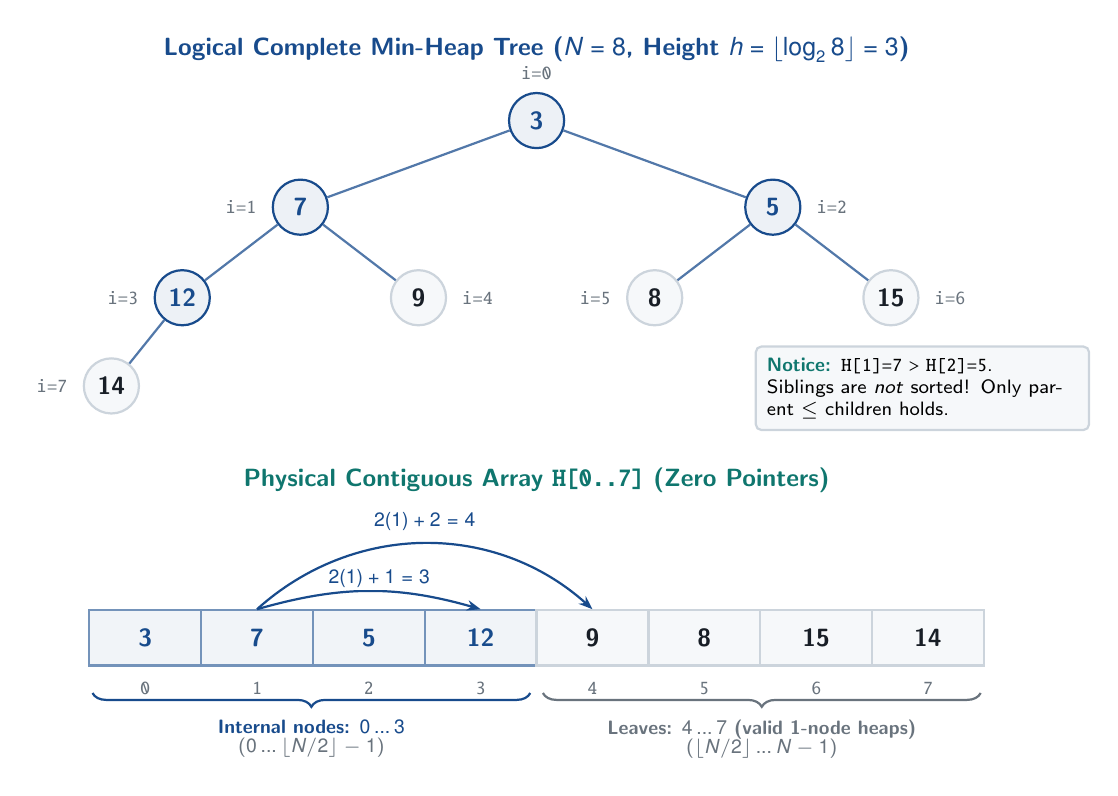
\begin{tikzpicture}[
    node/.style={circle, draw=primaryblue, fill=primaryblue!8, thick, minimum size=0.70cm, inner sep=0pt, font=\small\bfseries, text=primaryblue},
    leaf/.style={circle, draw=codeframe, fill=codebg, thick, minimum size=0.70cm, inner sep=0pt, font=\small\bfseries, text=codeink},
    cell/.style={draw=primaryblue!60, fill=primaryblue!6, thick, minimum width=1.42cm, minimum height=0.70cm, font=\small\bfseries, text=primaryblue},
    lcell/.style={draw=codeframe, fill=codebg, thick, minimum width=1.42cm, minimum height=0.70cm, font=\small\bfseries, text=codeink},
    idx/.style={font=\scriptsize\ttfamily\color{codegray}}
]
    % Title banner
    \node[font=\small\bfseries\color{primaryblue}] at (7.5, 6.05) {Logical Complete Min-Heap Tree ($N = 8$, Height $h = \lfloor \log_2 8 \rfloor = 3$)};

    % Tree nodes (centered at x=7.5)
    \node[node] (n0) at (7.5, 5.15) {3};
    \node[idx, above=1pt of n0] {i=0};

    \node[node] (n1) at (4.5, 4.05) {7};
    \node[idx, left=2pt of n1] {i=1};
    \node[node] (n2) at (10.5, 4.05) {5};
    \node[idx, right=2pt of n2] {i=2};

    \node[node] (n3) at (3.0, 2.90) {12};
    \node[idx, left=2pt of n3] {i=3};
    \node[leaf] (n4) at (6.0, 2.90) {9};
    \node[idx, right=2pt of n4] {i=4};
    \node[leaf] (n5) at (9.0, 2.90) {8};
    \node[idx, left=2pt of n5] {i=5};
    \node[leaf] (n6) at (12.0, 2.90) {15};
    \node[idx, right=2pt of n6] {i=6};

    \node[leaf] (n7) at (2.1, 1.78) {14};
    \node[idx, left=2pt of n7] {i=7};

    % Tree edges
    \draw[thick, primaryblue!75] (n0) -- (n1);
    \draw[thick, primaryblue!75] (n0) -- (n2);
    \draw[thick, primaryblue!75] (n1) -- (n3);
    \draw[thick, primaryblue!75] (n1) -- (n4);
    \draw[thick, primaryblue!75] (n2) -- (n5);
    \draw[thick, primaryblue!75] (n2) -- (n6);
    \draw[thick, primaryblue!75] (n3) -- (n7);

    % Note on sibling order
    \node[lmbox, align=left, text width=3.95cm, font=\scriptsize] at (12.4, 1.75) {
        \textbf{\color{accentteal}Notice:} \texttt{H[1]=7 > H[2]=5}.\\
        Siblings are \emph{not} sorted! Only parent $\le$ children holds.
    };

    % Divider label cleanly below Notice box and well above curved arcs
    \node[font=\small\bfseries\color{accentteal}] at (7.5, 0.58) {Physical Contiguous Array \texttt{H[0..7]} (Zero Pointers)};

    % Flat array strip
    \foreach \val/\i in {3/0, 7/1, 5/2, 12/3} {
        \pgfmathsetmacro{\xpos}{2.53 + \i*1.42}
        \node[cell] (a\i) at (\xpos, -1.42) {\val};
        \node[idx, below=2pt of a\i] {\i};
    }
    \foreach \val/\i in {9/4, 8/5, 15/6, 14/7} {
        \pgfmathsetmacro{\xpos}{2.53 + \i*1.42}
        \node[lcell] (a\i) at (\xpos, -1.42) {\val};
        \node[idx, below=2pt of a\i] {\i};
    }

    % Parent -> child arcs cleanly separated (outer arc drawn high first, inner arc low second)
    \draw[lmarrow, bend left=42] (a1.north) to node[above=1pt, font=\scriptsize\color{primaryblue}] {$2(1)+2=4$} (a4.north);
    \draw[lmarrow, bend left=16] (a1.north) to node[above=0pt, pos=0.55, fill=white, inner sep=1pt, font=\scriptsize\color{primaryblue}] {$2(1)+1=3$} (a3.north);

    % Braces below array with compact two-line centered labels (wide gutter)
    \draw[decorate, decoration={brace, amplitude=5pt, mirror}, thick, primaryblue]
        (1.86, -2.12) -- (7.42, -2.12)
        node[midway, below=6pt, align=center, font=\scriptsize\bfseries\color{primaryblue}] {Internal nodes: $0 \dots 3$\\[-1pt]\normalfont\color{codegray}($0 \dots \lfloor N/2 \rfloor - 1$)};
    \draw[decorate, decoration={brace, amplitude=5pt, mirror}, thick, codegray]
        (7.58, -2.12) -- (13.14, -2.12)
        node[midway, below=6pt, align=center, font=\scriptsize\bfseries\color{codegray}] {Leaves: $4 \dots 7$ (valid 1-node heaps)\\[-1pt]\normalfont($\lfloor N/2 \rfloor \dots N - 1$)};
\end{tikzpicture}
\caption{A complete binary min-heap and its exact 0-based contiguous array layout. Every level packs sequentially with zero gaps; indices $\lfloor N/2 \rfloor \dots N-1$ are always leaves.}
\label{fig:heap_array_layout}
\end{figure}

\begin{tryitbox}{Trace}{Array Indexing and Heap Validity}{ex1}
Consider the 0-based array \texttt{A = [2, 8, 5, 10, 9, 6, 7, 11, 14]} ($N = 9$).
\begin{enumerate}[itemsep=1pt, topsep=2pt]
    \item Without drawing pointers, compute $\text{parent}(7)$, $\text{left}(3)$, $\text{right}(3)$, and the index range of all leaves.
    \item Does \texttt{A} satisfy the min-heap invariant? Check every internal node, and note whether \texttt{A[1] > A[2]} breaks anything.
\end{enumerate}
\end{tryitbox}

% ============================================================================
\section{Heap Operations and Linear-Time Heapify}
% ============================================================================

Both dynamic updates (\texttt{push} and \texttt{pop}) follow the exact same design philosophy: \textbf{preserve completeness first} (always append or remove at the very last slot \texttt{N-1}), then repair the single local violation of heap order along one root-to-leaf path in $O(\log N)$.

% ----------------------------------------------------------------------------
\subsection{Push (\texttt{sift\_up}) and Pop (\texttt{sift\_down})}
% ----------------------------------------------------------------------------

\begin{notationbox}[Symbols Used Here]
\texttt{sift\_up(i)} & Bubbles element at $i$ upward until $\text{parent}(i) \le H[i]$ or $i = 0$ & Used by \texttt{push} \\
\texttt{sift\_down(i)} & Sinks element at $i$ downward, swapping with the \emph{smaller} child & Used by \texttt{pop}, heapify \\
$h = \lfloor \log_2 N \rfloor$ & Maximum number of levels an element can travel in either direction & Worst-case swaps $\le h$ \\
\end{notationbox}

\painbeat Inserting into the middle of an array shifts $O(N)$ elements, and deleting the root \texttt{H[0]} directly leaves a hole at the top of the tree that violates the complete-tree layout.

\ahabeat Every update touches the \emph{back} of the vector first (\texttt{push\_back} or swap root with \texttt{back()} and \texttt{pop\_back}), keeping the tree complete in $O(1)$. Only one node can now be out of order, so climbing up or sinking down repairs the entire heap in at most $\lfloor \log_2 N \rfloor$ swaps.

\examplebeat Look at Figure~\ref{fig:sift_up_down}:
\begin{itemize}
    \item \textbf{Push(\texttt{4})} onto \texttt{[3, 7, 5, 12, 9, 8, 15]}: Append \texttt{4} at index \texttt{7}. Compare with parent \texttt{H[3] = 12} (swap!), then parent \texttt{H[1] = 7} (swap!), then parent \texttt{H[0] = 3} ($4 \ge 3$, stop!). Result: \texttt{[3, 4, 5, 7, 9, 8, 15, 12]}.
    \item \textbf{Pop()} from \texttt{[3, 7, 5, 12, 9, 8, 15, 14]}: Save root \texttt{3}, move last leaf \texttt{14} into index \texttt{0}, shrink size to 7. Compare \texttt{14} against its two children \texttt{7} and \texttt{5}; pick the \emph{smaller} child \texttt{5} (index \texttt{2}) and swap! Now compare \texttt{14} against children \texttt{8} and \texttt{15}; swap with \texttt{8} (index \texttt{5}). No children remain, stop! Result: \texttt{[5, 7, 8, 12, 9, 14, 15]}.
\end{itemize}

\invariantbeat{Sift-Down} At the start of each step at index $i$, every subtree in the heap satisfies the min-heap property \emph{except possibly} the relationship between $H[i]$ and its immediate children.

\begin{watchoutbox}[Watch Out --- Always Swap with the \emph{Best} Child]
During min-heap \texttt{sift\_down}, suppose $H[0] = 14$ has children $7$ and $5$. If you carelessly swap $14$ with the \emph{first} smaller child you see ($7$) instead of the \emph{smallest} child ($5$), then $7$ becomes the parent of $5$ --- instantly breaking the heap invariant at the root! Always find \texttt{best = argmin(H[i], H[left], H[right])} before swapping.
\end{watchoutbox}

\begin{figure}[htbp]
\centering
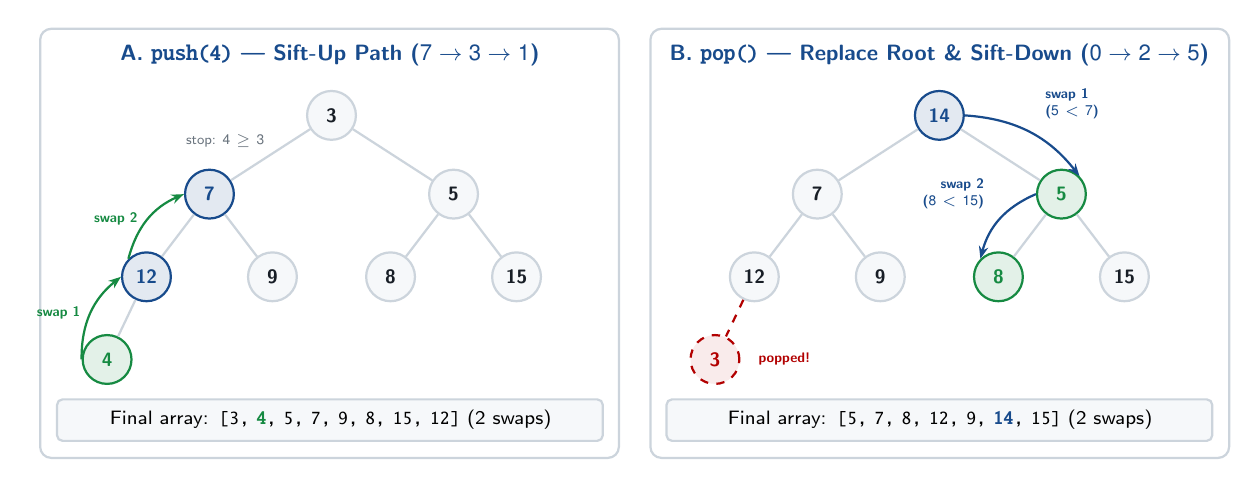
\begin{tikzpicture}[
    nrm/.style={circle, draw=codeframe, fill=codebg, thick, minimum size=0.62cm, inner sep=0pt, font=\scriptsize\bfseries, text=codeink},
    act/.style={circle, draw=primaryblue, fill=primaryblue!12, thick, minimum size=0.62cm, inner sep=0pt, font=\scriptsize\bfseries, text=primaryblue},
    acc/.style={circle, draw=codegreen, fill=codegreen!12, thick, minimum size=0.62cm, inner sep=0pt, font=\scriptsize\bfseries, text=codegreen},
    del/.style={circle, draw=red!70!black, fill=red!70!black!8, thick, dashed, minimum size=0.62cm, inner sep=0pt, font=\scriptsize\bfseries, text=red!70!black},
    lbl/.style={font=\tiny\ttfamily\color{codegray}}
]
    % Left Panel Box: Push / Sift-Up
    \draw[draw=codeframe, fill=white, rounded corners=4pt, thick] (0.0, 0.0) rectangle (7.35, 5.45);
    \node[font=\footnotesize\bfseries\color{primaryblue}] at (3.68, 5.12) {A. \texttt{push(4)} --- Sift-Up Path ($7 \to 3 \to 1$)};

    % Left Tree (centered at x=3.7)
    \node[nrm] (L0) at (3.70, 4.35) {3};
    \node[act] (L1) at (2.15, 3.35) {7};
    \node[nrm] (L2) at (5.25, 3.35) {5};
    \node[act] (L3) at (1.35, 2.30) {12};
    \node[nrm] (L4) at (2.95, 2.30) {9};
    \node[nrm] (L5) at (4.45, 2.30) {8};
    \node[nrm] (L6) at (6.05, 2.30) {15};
    \node[acc] (L7) at (0.85, 1.25) {4};

    \draw[thick, codeframe] (L0) -- (L1);
    \draw[thick, codeframe] (L0) -- (L2);
    \draw[thick, codeframe] (L1) -- (L3);
    \draw[thick, codeframe] (L1) -- (L4);
    \draw[thick, codeframe] (L2) -- (L5);
    \draw[thick, codeframe] (L2) -- (L6);
    \draw[thick, codeframe] (L3) -- (L7);

    % Sift-up swap arrows
    \draw[-{Stealth[length=4.5pt]}, thick, codegreen, bend left=26] (L7.west) to node[left, font=\tiny\bfseries\color{codegreen}] {swap 1} (L3.west);
    \draw[-{Stealth[length=4.5pt]}, thick, codegreen, bend left=26] (L3.north west) to node[left, font=\tiny\bfseries\color{codegreen}] {swap 2} (L1.west);
    \node[font=\tiny\color{codegray}, align=left] at (2.35, 4.02) {stop: $4 \ge 3$};

    \node[lmbox, align=center, text width=6.65cm, font=\scriptsize] at (3.68, 0.48) {
        Final array: \texttt{[3, \textcolor{codegreen}{\textbf{4}}, 5, 7, 9, 8, 15, 12]} (2 swaps)
    };

    % Right Panel Box: Pop / Sift-Down
    \draw[draw=codeframe, fill=white, rounded corners=4pt, thick] (7.75, 0.0) rectangle (15.10, 5.45);
    \node[font=\footnotesize\bfseries\color{primaryblue}] at (11.42, 5.12) {B. \texttt{pop()} --- Replace Root \& Sift-Down ($0 \to 2 \to 5$)};

    % Right Tree (centered at x=11.42)
    \node[act] (R0) at (11.42, 4.35) {14};
    \node[nrm] (R1) at (9.87, 3.35) {7};
    \node[acc] (R2) at (12.97, 3.35) {5};
    \node[nrm] (R3) at (9.07, 2.30) {12};
    \node[nrm] (R4) at (10.67, 2.30) {9};
    \node[acc] (R5) at (12.17, 2.30) {8};
    \node[nrm] (R6) at (13.77, 2.30) {15};
    \node[del] (R7) at (8.57, 1.25) {3};

    \draw[thick, codeframe] (R0) -- (R1);
    \draw[thick, codeframe] (R0) -- (R2);
    \draw[thick, codeframe] (R1) -- (R3);
    \draw[thick, codeframe] (R1) -- (R4);
    \draw[thick, codeframe] (R2) -- (R5);
    \draw[thick, codeframe] (R2) -- (R6);
    \draw[thick, dashed, red!70!black] (R3) -- (R7);

    \node[font=\tiny\bfseries\color{red!70!black}, right=3pt of R7] {popped!};

    % Sift-down swap arrows (labels pushed cleanly outside curved paths)
    \draw[-{Stealth[length=4.5pt]}, thick, primaryblue, bend left=24] (R0.east) to node[above right=1pt and 2pt, font=\tiny\bfseries\color{primaryblue}, align=left] {swap 1\\($5 < 7$)} (R2.north east);
    \draw[-{Stealth[length=4.5pt]}, thick, primaryblue, bend right=26] (R2.west) to node[above left=0pt and 2pt, font=\tiny\bfseries\color{primaryblue}, align=right] {swap 2\\($8 < 15$)} (R5.north west);

    \node[lmbox, align=center, text width=6.65cm, font=\scriptsize] at (11.42, 0.48) {
        Final array: \texttt{[5, 7, 8, 12, 9, \textcolor{primaryblue}{\textbf{14}}, 15]} (2 swaps)
    };
\end{tikzpicture}
\caption{Dynamic heap updates preserve completeness at index $N-1$ first, then repair heap order in $O(\log N)$ swaps. Left: \texttt{push(4)} bubbles upward. Right: \texttt{pop()} swaps root \texttt{3} with leaf \texttt{14}, removes \texttt{3}, and sinks \texttt{14} along the smaller child at each level.}
\label{fig:sift_up_down}
\end{figure}

\begin{tryitbox}{Trace}{Hand-Trace Push Then Pop}{ex2}
Start with the valid 6-element min-heap \texttt{H = [4, 9, 6, 15, 11, 8]}.
\begin{enumerate}[itemsep=1pt, topsep=2pt]
    \item Execute \texttt{push(2)} and write the exact array \texttt{H} and index swap path.
    \item From that updated 7-element heap, execute \texttt{pop()} (removing the minimum) and write the exact resulting 6-element array \texttt{H}.
\end{enumerate}
\end{tryitbox}

% ----------------------------------------------------------------------------
\subsection{Floyd's Bottom-Up Heapify: Why Building a Heap Is \texorpdfstring{$O(N)$}{O(N)}}
% ----------------------------------------------------------------------------

\begin{notationbox}[Symbols Used Here]
$n_h$ & Number of nodes at height $h$ (leaves have $h = 0$) & $n_h \le \lceil N / 2^{h+1} \rceil$ \\
$W(N)$ & Worst-case total \texttt{sift\_down} swaps across all $N$ nodes & $W(N) \le N - 1 < 2N$ \\
$\operatorname{popcount}(N)$ & Number of \texttt{1}-bits in the binary representation of $N$ & Exact sum: $N - \operatorname{popcount}(N)$ \\
\end{notationbox}

\painbeat Suppose you are handed an unsorted vector of $N$ numbers and want to turn it into a heap. Pushing them one by one calls \texttt{sift\_up} on every new leaf at depth $\approx \log_2 N$. On descending input, half of all $N$ nodes climb all the way to the root, costing $\Theta(N \log N)$ time.

\ahabeat Reverse the direction! Run \texttt{sift\_down} \textbf{bottom-up} from the last internal node $i = \lfloor N/2 \rfloor - 1$ down to $0$. Because \emph{most nodes live near the bottom of a binary tree}, half the nodes are leaves (height $0$: \textbf{zero} swaps), a quarter sit at height $1$ (at most 1 swap), an eighth sit at height $2$ (at most 2 swaps), and only the lone root can sink $\lfloor \log_2 N \rfloor$ steps!

\examplebeat Compare both methods on a perfect binary tree of $N = 15$ nodes (4 levels: 1 root, 2, 4, and 8 leaves):
\begin{itemize}
    \item \textbf{Top-down \texttt{sift\_up} worst case} (node at depth $d$ climbs at most $d$ edges):
    $$1 \cdot 0 + 2 \cdot 1 + 4 \cdot 2 + 8 \cdot 3 = 0 + 2 + 8 + 24 = \mathbf{34} \text{ swaps.}$$
    \item \textbf{Bottom-up \texttt{sift\_down} worst case} (node at height $h$ sinks at most $h$ edges):
    $$8 \cdot 0 + 4 \cdot 1 + 2 \cdot 2 + 1 \cdot 3 = 0 + 4 + 4 + 3 = \mathbf{11} \text{ swaps } (< N!).$$
\end{itemize}

\begin{formulabox}[Why Bottom-Up Heapify Is Strictly Linear $O(N)$]
In any $N$-node complete binary tree, at most $\lceil N / 2^{h+1} \rceil$ nodes sit at height $h \ge 1$. Since $h \le \lfloor \log_2 N \rfloor$ implies $x = N / 2^{h+1} \ge \frac{1}{2}$, we have $\lceil x \rceil \le 2x$, giving $\lceil N / 2^{h+1} \rceil \le N / 2^h$. Summing the max swaps $h$ over all heights:
$$W(N) \;\le\; \sum_{h=1}^{\lfloor \log_2 N \rfloor} \left\lceil \frac{N}{2^{h+1}} \right\rceil h \;\le\; N \sum_{h=1}^{\infty} \frac{h}{2^h} \;=\; 2N \;=\; O(N).$$
\textbf{Why does $\sum_{h=1}^{\infty} \frac{h}{2^h} = 2$?} Use the shift-and-subtract trick from Module~04! Let $S = \frac{1}{2} + \frac{2}{4} + \frac{3}{8} + \frac{4}{16} + \dots$, then $2S = 1 + \frac{2}{2} + \frac{3}{4} + \frac{4}{8} + \dots$; subtracting gives $2S - S = 1 + \frac{1}{2} + \frac{1}{4} + \frac{1}{8} + \dots = 2$. \emph{(Bonus exact identity: summing node heights over any complete binary tree equals exactly $N - \operatorname{popcount}(N) \le N - 1$ swaps, or at most $2N$ comparisons.)}
\end{formulabox}

\begin{watchoutbox}[Watch Out --- Direction Matters for \texttt{sift\_down}!]
Bottom-up heapify works \emph{only} because when \texttt{sift\_down(i)} runs, its left and right subtrees are \textbf{already valid heaps}. If you reverse the loop and call \texttt{sift\_down} top-down from $i = 0$ to $\lfloor N/2 \rfloor - 1$, deep small values never get lifted to the root --- on \texttt{[1, 2, 3, 4, 5, 6, 0]}, top-down \texttt{sift\_down} stops at \texttt{[1, 2, 0, 4, 5, 6, 3]}, leaving \texttt{0} trapped below \texttt{1}!
\end{watchoutbox}

\begin{tryitbox}{Derive}{Heapify Work Budget and Loop-Order Bug}{ex3}
\begin{enumerate}[itemsep=1pt, topsep=2pt]
    \item Compute the exact maximum \texttt{sift\_down} swap count $N - \operatorname{popcount}(N)$ vs.\ worst-case top-down \texttt{sift\_up} swap count for $N = 7$.
    \item Trace top-down \texttt{sift\_down} ($i = 0, 1, 2$) on \texttt{[1, 2, 3, 4, 5, 6, 0]} to verify which node ends up violating the min-heap property.
\end{enumerate}
\end{tryitbox}

% ============================================================================
\section{Core Heap Patterns}
% ============================================================================

Almost every priority-queue problem in algorithmic programming reduces to one of four reusable patterns: \textbf{Top-$K$}, \textbf{$K$-Way Merge}, \textbf{Two-Heap Median}, and \textbf{Lazy Deletion}.

% ----------------------------------------------------------------------------
\subsection{Top-\texorpdfstring{$K$}{K} Largest / Smallest Elements (The Inverted-Heap Trick)}
% ----------------------------------------------------------------------------

\begin{notationbox}[Symbols Used Here]
$N$ & Total number of items in the array or stream & Up to $10^7$ (streaming) \\
$K$ & Number of top items to retain ($1 \le K \le N$) & Often $K \ll N$ \\
$H_{\min}$ & Size-$K$ min-heap holding the $K$ largest items seen so far & Root = $K$-th largest item \\
\end{notationbox}

\painbeat Sorting an array of $N$ elements just to read the top $K$ largest values costs $O(N \log N)$ time and requires holding all $N$ items in RAM at once --- impossible for a live stream of $10^7$ events when you only want the top $K = 10$.

\ahabeat To track the \textbf{$K$ largest} items, use a \textbf{min-heap} of size $K$ (the \emph{opposite} polarity!). Think of it as a VIP room with $K$ seats: the root is the \emph{weakest} member currently inside. Any newcomer $\le \text{root}$ is rejected in $O(1)$; any newcomer $> \text{root}$ evicts the weakest member in $O(\log K)$.

\examplebeat Find the $K = 3$ largest values in \texttt{[4, 1, 9, 2, 7, 5, 8]}:
\begin{enumerate}[itemsep=2pt]
    \item Fill first $K = 3$ seats: push \texttt{4, 1, 9} $\to H_{\min} = [1, 4, 9]$ (root = \texttt{1}).
    \item See \texttt{2} $> 1$: evict \texttt{1}, push \texttt{2} $\to H_{\min} = [2, 4, 9]$.
    \item See \texttt{7} $> 2$: evict \texttt{2}, push \texttt{7} $\to H_{\min} = [4, 7, 9]$.
    \item See \texttt{5} $> 4$: evict \texttt{4}, push \texttt{5} $\to H_{\min} = [5, 7, 9]$.
    \item See \texttt{8} $> 5$: evict \texttt{5}, push \texttt{8} $\to H_{\min} = [7, 8, 9]$. Top 3 = $\{7, 8, 9\}$; $3^{\text{rd}}$ largest = root \texttt{7}!
\end{enumerate}

\begingroup\footnotesize\rowcolors{2}{codebg}{white}
\begin{tabularx}{\textwidth}{>{\raggedright\arraybackslash\bfseries}p{4.3cm} >{\centering\arraybackslash}p{2.2cm} >{\centering\arraybackslash}p{1.5cm} >{\raggedright\arraybackslash}X}
\arrayrulecolor{primaryblue}\toprule[1.2pt]
\rowcolor{primaryblue!10}
\textcolor{primaryblue}{\textbf{Top-$K$ Strategy}} & \textcolor{primaryblue}{\textbf{Time}} & \textcolor{primaryblue}{\textbf{Space}} & \textcolor{primaryblue}{\textbf{Best Regime}} \\
\arrayrulecolor{codeframe}\midrule[0.6pt]
Size-$K$ Min-Heap & $O(N \log K)$ & $O(K)$ & Streaming data or $K \ll N$ (low RAM). \\
Floyd Heapify + $K$ Pops & $O(N + K \log N)$ & $O(N)$ & Offline array with tiny $K$ (fast build). \\
\texttt{std::ranges::nth\_element} & $O(N)$ avg & $O(1)$ & Offline array needing unordered Top-$K$. \\
Full Sort & $O(N \log N)$ & $O(\log N)$ & Tiny $N$ or when full sorted order is needed. \\
\arrayrulecolor{primaryblue}\bottomrule[1.2pt]
\end{tabularx}\endgroup

\begin{watchoutbox}[Watch Out --- Inverted Polarity Trap]
Using a \textbf{max-heap} of size $K$ to find the $K$ \emph{largest} items is a classic bug: when the $(K+1)$-th element arrives, popping the root evicts the \textbf{global maximum}! Remember the rule: \textbf{Top-$K$ largest $\implies$ Min-Heap; Top-$K$ smallest $\implies$ Max-Heap.}
\end{watchoutbox}

\begin{tryitbox}{Twist}{K Closest Points to the Origin}{ex4}
You are given 5 points $(3, 4),\; (1, 3),\; (2, 2),\; (4, 1),\; (-1, 2)$ and want the $K = 2$ \textbf{closest} points to $(0, 0)$.
\begin{enumerate}[itemsep=1pt, topsep=2pt]
    \item Should you maintain a size-$2$ \textbf{min-heap} or \textbf{max-heap}, and why should you compare $x^2 + y^2$ instead of $\sqrt{x^2 + y^2}$?
    \item Trace the size-$2$ heap across all 5 points and list the final 2 closest points.
\end{enumerate}
\end{tryitbox}

% ----------------------------------------------------------------------------
\subsection{\texorpdfstring{$K$}{K}-Way Merge (Multi-Stream Frontier)}
% ----------------------------------------------------------------------------

\begin{notationbox}[Symbols Used Here]
$K$ & Number of individually sorted input lists $L_0, L_1, \dots, L_{K-1}$ & $K \ge 1$ \\
$N$ & Total number of elements across all $K$ lists ($N = \sum |L_r|$) & Output length \\
$(v, r, c)$ & Heap frontier tuple: value $v = L_r[c]$, list index $r$, element index $c$ & Ordered by $v$ \\
\end{notationbox}

\painbeat Suppose you must merge $K = 1{,}000$ sorted lists containing $N = 10^5$ total numbers. Merging lists sequentially (\texttt{merge(L0, L1)}, then merging the result with \texttt{L2}, and so on) re-copies elements from early lists up to $K$ times, costing $O(N \cdot K) \approx 10^8$ operations.

\ahabeat At any moment, the next globally smallest element \emph{must} be the unconsumed head of one of the $K$ sorted lists! Keep a min-heap of at most $K$ frontier entries $(L_r[c], r, c)$ --- one per non-empty list. Pop the smallest entry in $O(\log K)$ and immediately push its successor $(L_r[c+1], r, c+1)$ from that exact same list.

\examplebeat Merging 3 lists $L_0 = [1, 6, 11]$, $L_1 = [2, 5, 9]$, $L_2 = [3, 4, 12]$: start with frontier $\{(1, 0, 0),\; (2, 1, 0),\; (3, 2, 0)\}$. Pop $1$ from $L_0$ and push $(6, 0, 1)$; pop $2$ from $L_1$ and push $(5, 1, 1)$; pop $3$ from $L_2$ and push $(4, 2, 1)$. Every element enters and leaves the size-$K$ heap once, giving $O(N \log K)$ time and $O(K)$ auxiliary space!

\begin{calloutbox}{Disguised $K$-Way Merge Problems}
Many seemingly unrelated problems are $K$-way merges under the hood: \textbf{$K$-th Smallest Element in a Row-Sorted Matrix} (each row is a sorted list), \textbf{$K$ Pairs with Smallest Sums} from two sorted arrays $A, B$ (row $i$ is $A[i] + B[0], A[i] + B[1], \dots$), and \textbf{Smallest Range Covering at Least One Element from Each of $K$ Lists} (track the current max across the $K$-element min-heap frontier).
\end{calloutbox}

\begin{watchoutbox}[Watch Out --- Empty Lists and End-of-Stream Guards]
Always skip empty lists ($L_r.\text{empty}()$) during initial frontier loading, and check $c + 1 < |L_r|$ before pushing the next entry after each pop. Forgetting either check triggers an immediate out-of-bounds read.
\end{watchoutbox}

\begin{tryitbox}{Trace}{Multi-Stream Frontier Trace}{ex5}
Trace the first \textbf{5 pops} of $K$-way merge on the 3 sorted lists $L_0 = [2, 8]$, $L_1 = [1, 4, 9]$, and $L_2 = [3, 7]$. For each pop, write the popped tuple $(v, r, c)$, the newly pushed tuple (or ``none''), and the remaining heap frontier.
\end{tryitbox}

% ----------------------------------------------------------------------------
\subsection{Two-Heap Running Median (Balanced Dual Priority Queues)}
% ----------------------------------------------------------------------------

\begin{notationbox}[Symbols Used Here]
$L$ & \textbf{Max-heap} storing the smaller (lower) half of seen values & Root = $\max(L)$ \\
$U$ & \textbf{Min-heap} storing the larger (upper) half of seen values & Root = $\min(U)$ \\
$m$ & Current running median of all inserted elements & $\max(L)$ or $\frac{\max(L)+\min(U)}{2}$ \\
\end{notationbox}

\painbeat Given a live stream of numbers, finding the median after every arrival by re-sorting the prefix costs $O(N^2 \log N)$. Even keeping a sorted vector via binary search + insertion still shifts $O(N)$ elements per arrival ($O(N^2)$ total).

\ahabeat To compute a median, you do \emph{not} need either half sorted! You only need instant $O(1)$ access to the two numbers right at the middle boundary: the \textbf{largest element of the lower half} ($\max L$) and the \textbf{smallest element of the upper half} ($\min U$). Pairing a max-heap $L$ with a min-heap $U$ exposes both boundaries in $O(1)$ and updates in $O(\log N)$!

\begin{formulabox}[Two-Heap Running Median Invariants \& Median Formula]
Maintain two invariants after every \texttt{add(x)}:
\begin{enumerate}[itemsep=1pt, topsep=2pt]
    \item \textbf{Order invariant:} Every element in $L$ is $\le$ every element in $U$ (equivalently, $\max(L) \le \min(U)$ whenever both are non-empty).
    \item \textbf{Size invariant:} $|L| = |U|$ (even count) or $|L| = |U| + 1$ (odd count).
\end{enumerate}
Then the median is immediately:
$$m \;=\; \begin{cases} \max(L) & \text{if } |L| = |U| + 1, \\[3pt] \dfrac{\max(L) + \min(U)}{2} & \text{if } |L| = |U|. \end{cases}$$
\textbf{Zero-branching 3-step \texttt{add(x)} recipe:} (1) push $x$ into $L$; (2) pop $\max(L)$ and push it into $U$ \emph{(guarantees $\max(L) \le \min(U)$ automatically!)}; (3) if $|U| > |L|$, pop $\min(U)$ and push it back into $L$ \emph{(restores $|L| \in \{|U|, |U|+1\}$)}.
\end{formulabox}

\examplebeat Stream \texttt{[5, 2, 10, 4, 7]} using the 3-step recipe:
\begin{itemize}[itemsep=1pt]
    \item \texttt{add(5)}: $L=[5],\; U=[] \implies m = 5$.
    \item \texttt{add(2)}: push $2 \to L=[5,2]$; move $5 \to U=[5]$; $|L|=|U|=1 \implies m = (2+5)/2 = 3.5$.
    \item \texttt{add(10)}: push $10 \to L$; move $10 \to U=[5,10]$; $|U|>|L|$ so move $5 \to L=[5,2],\; U=[10] \implies m = 5$.
    \item \texttt{add(4)}: push $4 \to L$; move $5 \to U=[5,10]$; $L=[4,2],\; U=[5,10] \implies m = (4+5)/2 = 4.5$.
    \item \texttt{add(7)}: push $7 \to L$; move $7 \to U=[5,7,10]$; move $5 \to L=[5,4,2],\; U=[7,10] \implies m = 5$.
\end{itemize}

\begin{figure}[htbp]
\centering
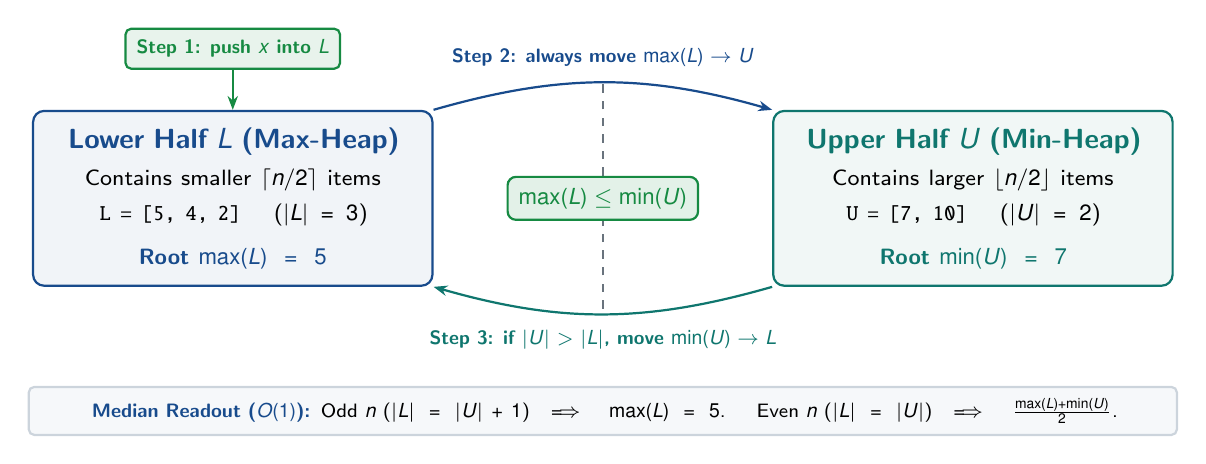
\begin{tikzpicture}[
    hcard/.style={draw=primaryblue, fill=primaryblue!6, thick, rounded corners=4pt, align=center, text width=4.65cm, inner sep=6pt},
    rcard/.style={draw=accentteal, fill=accentteal!6, thick, rounded corners=4pt, align=center, text width=4.65cm, inner sep=6pt},
    badge/.style={draw=codegreen, fill=codegreen!12, thick, rounded corners=3pt, font=\footnotesize\bfseries, text=codegreen, inner sep=4pt}
]
    % Left Heap Card (Max-Heap L) raised for generous bottom clearance
    \node[hcard] (Lbox) at (2.85, 3.05) {
        \textbf{\color{primaryblue}Lower Half $L$ (Max-Heap)}\\[4pt]
        \footnotesize Contains smaller $\lceil n/2 \rceil$ items\\[3pt]
        \texttt{L = [5, 4, 2]} \quad ($|L| = 3$)\\[4pt]
        \textbf{\color{primaryblue}Root $\max(L) = 5$}
    };

    % Right Heap Card (Min-Heap U)
    \node[rcard] (Ubox) at (12.25, 3.05) {
        \textbf{\color{accentteal}Upper Half $U$ (Min-Heap)}\\[4pt]
        \footnotesize Contains larger $\lfloor n/2 \rfloor$ items\\[3pt]
        \texttt{U = [7, 10]} \quad ($|U| = 2$)\\[4pt]
        \textbf{\color{accentteal}Root $\min(U) = 7$}
    };

    % Center Boundary Divider & Median Badge
    \draw[dashed, thick, codegray] (7.55, 1.65) -- (7.55, 4.55);
    \node[badge] (med) at (7.55, 3.05) {$\max(L) \le \min(U)$};

    % Transfer arrows (Step 2 and Step 3) with generous clearance from bottom box
    \draw[-{Stealth[length=5pt]}, thick, primaryblue, bend left=16]
        (Lbox.north east) to node[above=2pt, font=\scriptsize\bfseries\color{primaryblue}] {Step 2: always move $\max(L) \to U$} (Ubox.north west);
    \draw[-{Stealth[length=5pt]}, thick, accentteal, bend left=16]
        (Ubox.south west) to node[below=2pt, font=\scriptsize\bfseries\color{accentteal}] {Step 3: if $|U| > |L|$, move $\min(U) \to L$} (Lbox.south east);

    % Incoming arrow into L
    \node[lmaccepted, font=\scriptsize\bfseries] (inc) at (2.85, 4.95) {Step 1: push $x$ into $L$};
    \draw[-{Stealth[length=5pt]}, thick, codegreen] (inc.south) -- (Lbox.north);

    % Bottom Summary Strip cleanly separated below Step 3 label
    \node[lmbox, align=center, text width=14.3cm, font=\scriptsize] at (7.55, 0.35) {
        \textbf{\color{primaryblue}Median Readout ($O(1)$):} Odd $n$ ($|L| = |U| + 1$) $\implies \max(L) = 5$. \quad Even $n$ ($|L| = |U|$) $\implies \frac{\max(L) + \min(U)}{2}$.
    };
\end{tikzpicture}
\caption{Two-Heap Running Median architecture. Routing every incoming value through $L \to U$ (and balancing back only when $|U| > |L|$) guarantees both the order invariant $\max(L) \le \min(U)$ and the size invariant without error-prone \texttt{if/else} branching.}
\label{fig:two_heap_median}
\end{figure}

\begin{watchoutbox}[Watch Out --- Overflow and Ordering Violations]
Never route purely by size (pushing into $L$ when $|L| \le |U|$ and directly into $U$ otherwise): a huge element pushed directly into $L$ can exceed $\min(U)$! Also, when $n$ is even and inputs can reach $\pm 2 \times 10^9$, computing \texttt{(a + b) / 2.0} in 32-bit \texttt{int} overflows before conversion --- cast to \texttt{double} (or \texttt{std::int64\_t}) first, or compute \texttt{a + (b - a) / 2.0}.
\end{watchoutbox}

\begin{tryitbox}{Debug}{Broken Two-Heap Insert}{ex6}
A programmer writes a ``shortcut'' for \texttt{RunningMedian::add(int x)}:
\begin{quote}
\texttt{if (L.size() <= U.size()) L.push(x); else U.push(x);}
\end{quote}
Construct the \textbf{smallest} input stream (3 integers) where this code returns the wrong median, and explain which of the two invariants it breaks.
\end{tryitbox}

% ----------------------------------------------------------------------------
\subsection{Lazy Deletion Heap (Arbitrary Removals Without Pointers)}
% ----------------------------------------------------------------------------

\begin{notationbox}[Symbols Used Here]
\texttt{delayed[v]} & Hash map counting how many copies of value $v$ are marked deleted & \texttt{unordered\_map<int64\_t, int>} \\
\texttt{live\_L, live\_U} & Count of \textbf{active} (non-deleted) elements in $L$ and $U$ & Distinct from \texttt{.size()}! \\
\texttt{prune(H)} & Pops tombstones sitting at \texttt{H.top()} while \texttt{delayed[H.top()] > 0} & Amortized $O(\log N)$ \\
\end{notationbox}

\painbeat Suppose you want the \textbf{Sliding Window Median} over every contiguous subarray of length $K$. Unlike a growing stream, the oldest element $A[i - K]$ must be \emph{deleted} at every step. Standard \texttt{std::priority\_queue} has no \texttt{erase(value)} method because locating an arbitrary value inside an array heap takes $O(N)$!

\ahabeat You do \emph{not} need to dig an arbitrary element out of the middle of a heap --- while it sits buried below the root, it cannot affect \texttt{top()} at all! Simply record a tombstone \texttt{delayed[v]++} in a hash map and decrement the logical active counter \texttt{live}. Whenever a tombstone eventually floats to \texttt{H.top()}, \texttt{prune(H)} pops it in a \texttt{while} loop and decrements \texttt{delayed[v]}.

Because every inserted element is popped at most once over the entire run, all pruning work across $N$ slides amortizes to $O(N \log N)$ total (or $O(N \log K)$ if periodically compacted when physical size exceeds $2K$).

\examplebeat Watch \texttt{arr = [4, 1, 3, 5, 2, 6]} with $K = 3$:
\begin{itemize}[itemsep=1pt]
    \item Initial window \texttt{[4, 1, 3]}: $L = [3, 1]$ (\texttt{live}=2), $U = [4]$ (\texttt{live}=1) $\implies m = 3$.
    \item Slide \texttt{+5, -4} (\texttt{[1, 3, 5]}): \texttt{5} enters $U$; \texttt{4} leaves $U$ and sits right at \texttt{U.top()}, so \texttt{prune(U)} pops \texttt{4} immediately $\implies m = 3$.
    \item Slide \texttt{+2, -1} (\texttt{[3, 5, 2]}): \texttt{2} enters $L$; \texttt{1} leaves $L$ (\texttt{delayed[1]=1}), but \texttt{1} is \textbf{buried} beneath \texttt{3} and \texttt{2}! Physical \texttt{L.size()} is $3$, yet \texttt{live\_L} is $2$ $\implies m = 3$.
    \item Slide \texttt{+6, -3} (\texttt{[5, 2, 6]}): \texttt{6} enters $U$; \texttt{3} leaves $L$ and is pruned from \texttt{L.top()}; rebalance moves \texttt{5} from $U$ to $L$ ($L = [5, 2, 1_{\text{dead}}]$ with \texttt{live\_L}=2, $U=[6]$) $\implies m = 5$.
\end{itemize}

\begin{figure}[htbp]
\centering
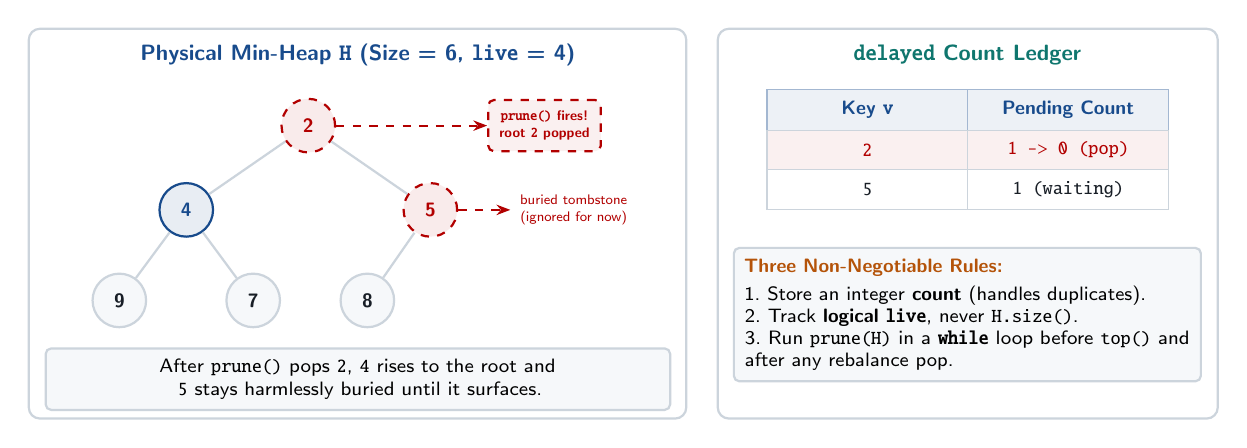
\begin{tikzpicture}[
    live/.style={circle, draw=primaryblue, fill=primaryblue!10, thick, minimum size=0.68cm, inner sep=0pt, font=\scriptsize\bfseries, text=primaryblue},
    liveleaf/.style={circle, draw=codeframe, fill=codebg, thick, minimum size=0.68cm, inner sep=0pt, font=\scriptsize\bfseries, text=codeink},
    dead/.style={circle, draw=red!70!black, fill=red!70!black!8, thick, dashed, minimum size=0.68cm, inner sep=0pt, font=\scriptsize\bfseries, text=red!70!black},
    panel/.style={draw=codeframe, fill=white, rounded corners=4pt, thick}
]
    % Left Panel: Min-Heap with buried tombstones (shifted slightly left for clean callout arrows)
    \draw[panel] (0.0, 0.0) rectangle (8.35, 4.95);
    \node[font=\footnotesize\bfseries\color{primaryblue}] at (4.18, 4.62) {Physical Min-Heap \texttt{H} (Size = 6, \texttt{live} = 4)};

    % Nodes
    \node[dead] (H0) at (3.55, 3.72) {2};
    \node[live] (H1) at (2.00, 2.65) {4};
    \node[dead] (H2) at (5.10, 2.65) {5};
    \node[liveleaf] (H3) at (1.15, 1.50) {9};
    \node[liveleaf] (H4) at (2.85, 1.50) {7};
    \node[liveleaf] (H5) at (4.30, 1.50) {8};

    \draw[thick, codeframe] (H0) -- (H1);
    \draw[thick, codeframe] (H0) -- (H2);
    \draw[thick, codeframe] (H1) -- (H3);
    \draw[thick, codeframe] (H1) -- (H4);
    \draw[thick, codeframe] (H2) -- (H5);

    % Annotations with clean horizontal clearance
    \node[lmpruned, font=\tiny\bfseries, align=center] (gate) at (6.55, 3.72) {\texttt{prune()} fires!\\root \texttt{2} popped};
    \draw[lmprunedarrow] (H0.east) -- (gate.west);

    \node[font=\tiny\color{red!70!black}, align=center] (buried) at (6.92, 2.65) {buried tombstone\\(ignored for now)};
    \draw[lmprunedarrow] (H2.east) -- (buried.west);

    \node[lmbox, align=center, text width=7.65cm, font=\scriptsize] at (4.18, 0.50) {
        After \texttt{prune()} pops \texttt{2}, \texttt{4} rises to the root and \texttt{5} stays harmlessly buried until it surfaces.
    };

    % Right Panel: Delayed Map & Contract
    \draw[panel] (8.75, 0.0) rectangle (15.10, 4.95);
    \node[font=\footnotesize\bfseries\color{accentteal}] at (11.92, 4.62) {\texttt{delayed} Count Ledger};

    % Mini ledger table inside TikZ
    \node[draw=primaryblue!40, fill=primaryblue!8, minimum width=2.55cm, minimum height=0.52cm, font=\scriptsize\bfseries, text=primaryblue] (th1) at (10.65, 3.92) {Key \texttt{v}};
    \node[draw=primaryblue!40, fill=primaryblue!8, minimum width=2.55cm, minimum height=0.52cm, font=\scriptsize\bfseries, text=primaryblue] (th2) at (13.20, 3.92) {Pending Count};

    \node[draw=codeframe, fill=red!70!black!6, minimum width=2.55cm, minimum height=0.50cm, font=\scriptsize\ttfamily, text=red!70!black] at (10.65, 3.41) {2};
    \node[draw=codeframe, fill=red!70!black!6, minimum width=2.55cm, minimum height=0.50cm, font=\scriptsize\ttfamily, text=red!70!black] at (13.20, 3.41) {1 -> 0 (pop)};

    \node[draw=codeframe, fill=white, minimum width=2.55cm, minimum height=0.50cm, font=\scriptsize\ttfamily, text=codeink] at (10.65, 2.91) {5};
    \node[draw=codeframe, fill=white, minimum width=2.55cm, minimum height=0.50cm, font=\scriptsize\ttfamily, text=codeink] at (13.20, 2.91) {1 (waiting)};

    \node[lmbox, align=left, text width=5.65cm, font=\scriptsize] at (11.92, 1.32) {
        \textbf{\color{accentamber}Three Non-Negotiable Rules:}\\[2pt]
        1.\ Store an integer \textbf{count} (handles duplicates).\\
        2.\ Track \textbf{logical \texttt{live}}, never \texttt{H.size()}.\\
        3.\ Run \texttt{prune(H)} in a \textbf{\texttt{while}} loop before \texttt{top()} and after any rebalance pop.
    };
\end{tikzpicture}
\caption{Lazy Deletion Heap. Arbitrary deletions only increment \texttt{delayed[v]} and decrement \texttt{live} in $O(1)$; dead tombstones (dashed red) are discarded strictly at the root by \texttt{prune()}.}
\label{fig:lazy_deletion}
\end{figure}

\begin{watchoutbox}[Watch Out --- Logical Size vs. Physical Size]
In a Dual Lazy-Deletion Heap, rebalancing on \texttt{L.size()} instead of \texttt{live\_L} is a silent disaster: if $L$ holds 3 dead tombstones and 2 live values while $U$ holds 2 live values, physical sizes say $5$ vs.\ $2$ and push live items out of $L$ into $U$, corrupting every subsequent median! Also remember to call \texttt{prune()} \emph{before} rebalancing so you never transfer a tombstone across heaps, and \emph{again} after rebalancing in case the pop uncovered a buried tombstone.
\end{watchoutbox}

\begin{tryitbox}{Edge Cases}{Duplicates and Cascading Tombstones}{ex7}
Suppose a single Lazy-Deletion Min-Heap starts with \texttt{[1, 3, 3, 5]} (\texttt{live = 4}). We call \texttt{lazy\_delete(3)}, \texttt{lazy\_delete(3)}, and then \texttt{pop()} (which removes \texttt{1}).
\begin{enumerate}[itemsep=1pt, topsep=2pt]
    \item What must \texttt{top()} return after \texttt{pop()}?
    \item Explain the exact wrong answer you get if (a) \texttt{delayed} is an \texttt{unordered\_set<int>} (boolean) instead of a count map, or (b) \texttt{prune()} uses \texttt{if} instead of \texttt{while}.
\end{enumerate}
\end{tryitbox}

% ============================================================================
\section{C++23 Priority Queues and Comparators}
% ============================================================================

Knowing the data structure is only half the battle; C++'s standard library has two notorious sharp edges around heaps that trip up even experienced engineers.

% ----------------------------------------------------------------------------
\subsection{Comparator Polarity: Why \texttt{std::priority\_queue} Feels Backwards}
% ----------------------------------------------------------------------------

In \texttt{std::sort(v.begin(), v.end(), cmp)}, returning \texttt{true} for \texttt{cmp(a, b)} puts \texttt{a} \emph{before} \texttt{b} (closer to index \texttt{0}). In \texttt{std::priority\_queue<T, Container, Compare>}, the default comparator is \texttt{std::less<T>}, yet it creates a \textbf{max-heap}!

Why? Because \texttt{std::priority\_queue} puts the ``highest'' element at \texttt{top()} --- the element that would sit at the \emph{back} of a sorted range. Memorize one clean rule:
\begin{center}
\textbf{\color{primaryblue}\texttt{cmp(a, b) == true} means ``\texttt{a} has \emph{lower} priority than \texttt{b}'' (\texttt{b} rises above \texttt{a}).}
\end{center}

\begingroup\small\rowcolors{2}{codebg}{white}
\begin{tabularx}{\textwidth}{>{\raggedright\arraybackslash\bfseries}p{3.9cm} >{\raggedright\arraybackslash}p{4.4cm} >{\raggedright\arraybackslash}X}
\arrayrulecolor{primaryblue}\toprule[1.2pt]
\rowcolor{primaryblue!10}
\textcolor{primaryblue}{\textbf{Goal}} & \textcolor{primaryblue}{\textbf{Declaration}} & \textcolor{primaryblue}{\textbf{Who Sits at \texttt{top()}?}} \\
\arrayrulecolor{codeframe}\midrule[0.6pt]
Max-Heap (default) & \texttt{std::priority\_queue<int>} & Largest \texttt{int} (\texttt{std::less<>}: smaller sinks). \\
Min-Heap & \texttt{std::priority\_queue<int, std::vector<int>, std::greater<>>} & Smallest \texttt{int} (\texttt{std::greater<>}: larger sinks). \\
Custom Struct Min-Heap & \texttt{struct Cmp \{ bool operator()(const Job\& a, const Job\& b) const \{ return a.cost > b.cost; \} \};} & Smallest \texttt{cost} (higher \texttt{cost} has lower priority). \\
\arrayrulecolor{primaryblue}\bottomrule[1.2pt]
\end{tabularx}\endgroup

\begin{watchoutbox}[Watch Out --- Strict Weak Ordering Is Mandatory (Never Use \texttt{<=})]
Your comparator \textbf{must} satisfy Strict Weak Ordering: in particular, \texttt{cmp(x, x)} must \textbf{always} be \texttt{false}! Writing \texttt{return a.cost >= b.cost;} instead of \texttt{>} causes \textbf{Undefined Behavior} --- standard library \texttt{push\_heap}/\texttt{pop\_heap} loops can walk past index \texttt{0} and segfault on duplicate keys.
\end{watchoutbox}

% ----------------------------------------------------------------------------
\subsection{Free-Function Heap Algorithms (\texttt{std::ranges::make\_heap})}
% ----------------------------------------------------------------------------

Sometimes \texttt{std::priority\_queue} is too restrictive because it hides the underlying \texttt{std::vector} (you cannot iterate over its elements or reserve capacity directly without passing a pre-allocated vector). The \texttt{<algorithm>} header exposes the exact same binary-heap primitives directly on any random-access range:
\begin{itemize}
    \item \texttt{std::ranges::make\_heap(v, cmp)}: Floyd's bottom-up heapify in-place in \textbf{$O(N)$} time! (Note: the range constructor \texttt{std::priority\_queue<int> pq(v.begin(), v.end());} also calls \texttt{make\_heap} in $O(N)$.)
    \item \texttt{v.push\_back(x); std::ranges::push\_heap(v, cmp);}: Sifts the newly appended last element up in $O(\log N)$.
    \item \texttt{std::ranges::pop\_heap(v, cmp); auto top = v.back(); v.pop\_back();}: Moves the root to \texttt{v.back()} and sifts down the remaining $N - 1$ elements in $O(\log N)$.
    \item \texttt{std::ranges::sort\_heap(v, cmp)}: Repeatedly calls \texttt{pop\_heap} to sort \texttt{v} in-place (\textbf{Heapsort}: $O(N \log N)$ guaranteed worst-case, $O(1)$ extra space, non-stable).
\end{itemize}

% ----------------------------------------------------------------------------
\subsection{Heap vs. Balanced BST (\texttt{std::multiset}) vs. Monotonic Deque}
% ----------------------------------------------------------------------------

Do not force a binary heap where a sibling data structure wins outright:

\begingroup\small\rowcolors{2}{codebg}{white}
\begin{tabularx}{\textwidth}{>{\raggedright\arraybackslash\bfseries}p{3.6cm} >{\raggedright\arraybackslash}p{4.3cm} >{\raggedright\arraybackslash}X}
\arrayrulecolor{primaryblue}\toprule[1.2pt]
\rowcolor{primaryblue!10}
\textcolor{primaryblue}{\textbf{Need in Problem}} & \textcolor{primaryblue}{\textbf{Best Data Structure}} & \textcolor{primaryblue}{\textbf{Why}} \\
\arrayrulecolor{codeframe}\midrule[0.6pt]
Dynamic min/max only & \textbf{Binary Heap} (\texttt{priority\_queue}) & Lowest constant factor, contiguous RAM, $O(N)$ bulk build. \\
Sliding window \textbf{min/max} & \textbf{Monotonic Deque} (Module~11) & Strictly $O(N)$ total vs.\ $O(N \log K)$ for a lazy heap. \\
Sliding window \textbf{median} & \textbf{Two Heaps + Lazy Delete} (or \texttt{multiset}) & Deque cannot track the middle; dual heaps beat tree allocations. \\
Need \texttt{lower\_bound} or arbitrary \texttt{erase} & \textbf{Balanced BST} (\texttt{std::set} / \texttt{multiset}) & Supports ordered iteration, predecessor/successor, and $O(\log N)$ erase by iterator. \\
\arrayrulecolor{primaryblue}\bottomrule[1.2pt]
\end{tabularx}\endgroup

\begin{tryitbox}{Triage}{Pick the Right Extremum Structure}{ex8}
Choose the single best data structure (\textbf{Binary Heap}, \textbf{Monotonic Deque}, \textbf{\texttt{std::multiset}}, or \textbf{\texttt{std::ranges::nth\_element}}) for each task ($N = 2 \times 10^5$):
\begin{enumerate}[itemsep=1pt, topsep=2pt]
    \item Return the maximum value in every contiguous subarray of length $K = 1{,}000$.
    \item Process $N$ events: either insert a stock price, delete an exact price by ID, or query the \emph{smallest price strictly greater than} $X$.
    \item Given a static offline array of $N$ salaries, output the $500$ highest salaries in any order as fast as possible.
\end{enumerate}
\end{tryitbox}

% ============================================================================
\section{Worked Examples}
% ============================================================================

Every example below is traced completely step by step so you can reproduce it on scratch paper.

\begin{example}[Bottom-Up Floyd Heapify on 8 Elements]
Convert \texttt{H = [18, 9, 14, 7, 12, 3, 5, 2]} ($N = 8$) into a min-heap in-place using Floyd's bottom-up algorithm.

\textbf{Step 1 --- Find the last internal node:} $\lfloor N / 2 \rfloor - 1 = \lfloor 8 / 2 \rfloor - 1 = 3$. Indices \texttt{4..7} (\texttt{12, 3, 5, 2}) are leaves and need zero work.

\textbf{Step 2 --- Run \texttt{sift\_down(i)} for $i = 3, 2, 1, 0$:}
\begin{enumerate}[itemsep=1pt, topsep=2pt]
    \item $i = 3$ (\texttt{H[3] = 7}): only child is \texttt{left(3) = 7} (\texttt{2}). Swap \texttt{7} and \texttt{2} (1 swap).\\
    $\to$ \texttt{H = [18, 9, 14, 2, 12, 3, 5, 7]}.
    \item $i = 2$ (\texttt{H[2] = 14}): children are \texttt{H[5] = 3} and \texttt{H[6] = 5}; smaller is \texttt{3}. Swap \texttt{14} and \texttt{3} (1 swap).\\
    $\to$ \texttt{H = [18, 9, 3, 2, 12, 14, 5, 7]}.
    \item $i = 1$ (\texttt{H[1] = 9}): children are \texttt{H[3] = 2} and \texttt{H[4] = 12}; swap with \texttt{2}. Now at $i = 3$, only child \texttt{H[7] = 7} $< 9$; swap with \texttt{7} (2 swaps).\\
    $\to$ \texttt{H = [18, 2, 3, 7, 12, 14, 5, 9]}.
    \item $i = 0$ (\texttt{H[0] = 18}): children \texttt{2, 3} $\to$ swap with \texttt{2} ($i=1$); children \texttt{7, 12} $\to$ swap with \texttt{7} ($i=3$); child \texttt{9} $\to$ swap with \texttt{9} ($i=7$) (3 swaps).\\
    $\to$ \texttt{H = [2, 7, 3, 9, 12, 14, 5, 18]}.
\end{enumerate}

\textbf{Verification:} Every parent is $\le$ its children ($2 \le 7, 3$; $7 \le 9, 12$; $3 \le 14, 5$; $9 \le 18$). Total swaps: $1 + 1 + 2 + 3 = 7 = N - \operatorname{popcount}(8) = 8 - 1$.
\end{example}

\begin{example}[Top-$K$ Frequent Elements via Size-$K$ Min-Heap]
Find the $K = 2$ most frequent integers in \texttt{A = [5, 2, 5, 3, 5, 2, 1, 3, 5, 2, 4]}.

\textbf{Step 1 --- Tally frequencies ($O(N)$):}
$$\texttt{1} \mapsto 1,\quad \texttt{2} \mapsto 3,\quad \texttt{3} \mapsto 2,\quad \texttt{4} \mapsto 1,\quad \texttt{5} \mapsto 4.$$

\textbf{Step 2 --- Stream \texttt{(freq, val)} pairs through a size-$2$ min-heap:}
\begin{enumerate}[itemsep=1pt, topsep=2pt]
    \item \texttt{(1, 1)}: heap size $< 2 \implies$ push. Heap: \texttt{[(1, 1)]}.
    \item \texttt{(3, 2)}: heap size $< 2 \implies$ push. Heap: \texttt{[(1, 1), (3, 2)]} (root has freq $1$).
    \item \texttt{(2, 3)}: freq $2 > 1 \implies$ evict \texttt{(1, 1)}, push \texttt{(2, 3)}. Heap: \texttt{[(2, 3), (3, 2)]}.
    \item \texttt{(1, 4)}: freq $1 \le 2 \implies$ reject immediately in $O(1)$. Heap unchanged.
    \item \texttt{(4, 5)}: freq $4 > 2 \implies$ evict \texttt{(2, 3)}, push \texttt{(4, 5)}. Heap: \texttt{[(3, 2), (4, 5)]}.
\end{enumerate}

\textbf{Answer:} Popping remaining entries gives values \texttt{5} (freq 4) and \texttt{2} (freq 3). Total time: $O(N + U \log K)$ where $U$ is the number of distinct values.
\end{example}

\begin{example}[$K$-Way Merge of Three Sorted Streams]
Merge $L_0 = [1, 7, 10]$, $L_1 = [2, 5, 11]$, and $L_2 = [3, 6, 8]$ using a min-heap of tuples \texttt{(val, list, idx)}.

\textbf{Initial frontier:} \texttt{\{(1, 0, 0), (2, 1, 0), (3, 2, 0)\}}.

\begingroup\footnotesize\rowcolors{2}{codebg}{white}
\begin{tabularx}{\textwidth}{>{\centering\arraybackslash}p{0.8cm} >{\raggedright\arraybackslash}p{2.1cm} >{\raggedright\arraybackslash}p{2.25cm} >{\raggedright\arraybackslash}X >{\raggedright\arraybackslash}p{3.25cm}}
\arrayrulecolor{primaryblue}\toprule[1.1pt]
\rowcolor{primaryblue!10}
\textcolor{primaryblue}{\textbf{Step}} & \textcolor{primaryblue}{\textbf{Popped Min}} & \textcolor{primaryblue}{\textbf{Pushed Next}} & \textcolor{primaryblue}{\textbf{Frontier After Step}} & \textcolor{primaryblue}{\textbf{Output Prefix}} \\
\arrayrulecolor{codeframe}\midrule[0.6pt]
1 & \texttt{(1, L0, 0)} & \texttt{(7, L0, 1)} & \texttt{(2,L1,0), (3,L2,0), (7,L0,1)} & \texttt{[1]} \\
2 & \texttt{(2, L1, 0)} & \texttt{(5, L1, 1)} & \texttt{(3,L2,0), (5,L1,1), (7,L0,1)} & \texttt{[1, 2]} \\
3 & \texttt{(3, L2, 0)} & \texttt{(6, L2, 1)} & \texttt{(5,L1,1), (6,L2,1), (7,L0,1)} & \texttt{[1, 2, 3]} \\
4 & \texttt{(5, L1, 1)} & \texttt{(11, L1, 2)} & \texttt{(6,L2,1), (7,L0,1), (11,L1,2)} & \texttt{[1, 2, 3, 5]} \\
5 & \texttt{(6, L2, 1)} & \texttt{(8, L2, 2)} & \texttt{(7,L0,1), (8,L2,2), (11,L1,2)} & \texttt{[1, 2, 3, 5, 6]} \\
6 & \texttt{(7, L0, 1)} & \texttt{(10, L0, 2)} & \texttt{(8,L2,2), (10,L0,2), (11,L1,2)} & \texttt{[1, 2, 3, 5, 6, 7]} \\
7 & \texttt{(8, L2, 2)} & \emph{none} ($L_2$ done) & \texttt{(10,L0,2), (11,L1,2)} & \texttt{[..., 7, 8]} \\
8 & \texttt{(10, L0, 2)} & \emph{none} ($L_0$ done) & \texttt{(11,L1,2)} & \texttt{[..., 8, 10]} \\
9 & \texttt{(11, L1, 2)} & \emph{none} ($L_1$ done) & \texttt{\{\}} & \texttt{[1, 2, 3, 5, 6, 7, 8, 10, 11]} \\
\arrayrulecolor{primaryblue}\bottomrule[1.1pt]
\end{tabularx}\endgroup

\par\noindent Notice the heap never exceeds size $K = 3$, even if each list held a million records.
\end{example}

\begin{example}[Two-Heap Running Median]
Maintain the running median of the stream \texttt{[12, 4, 8, 15, 2, 10]} using the 3-step insert rule (push $L$, move $\max(L) \to U$, rebalance if $|U| > |L|$).

\begingroup\footnotesize\rowcolors{2}{codebg}{white}
\begin{tabularx}{\textwidth}{>{\centering\arraybackslash}p{1.2cm} >{\raggedright\arraybackslash}X >{\raggedright\arraybackslash}p{2.7cm} >{\raggedright\arraybackslash}p{2.7cm} >{\centering\arraybackslash}p{1.5cm}}
\arrayrulecolor{primaryblue}\toprule[1.1pt]
\rowcolor{primaryblue!10}
\textcolor{primaryblue}{\textbf{Input}} & \textcolor{primaryblue}{\textbf{3-Step Action}} & \textcolor{primaryblue}{\textbf{$L$ (Max-Heap)}} & \textcolor{primaryblue}{\textbf{$U$ (Min-Heap)}} & \textcolor{primaryblue}{\textbf{Median}} \\
\arrayrulecolor{codeframe}\midrule[0.6pt]
\texttt{12} & Push $12 \to L$; move $12 \to U$; $|U|>|L|$ move $12 \to L$. & \texttt{[12]} & \texttt{[]} & $12$ \\
\texttt{4} & Push $4 \to L$; move $12 \to U$; $|L|=|U|=1$. & \texttt{[4]} & \texttt{[12]} & $8.0$ \\
\texttt{8} & Push $8 \to L$; move $8 \to U$; $|U|>|L|$ move $8 \to L$. & \texttt{[8, 4]} & \texttt{[12]} & $8$ \\
\texttt{15} & Push $15 \to L$; move $15 \to U$; $|L|=|U|=2$. & \texttt{[8, 4]} & \texttt{[12, 15]} & $10.0$ \\
\texttt{2} & Push $2 \to L$; move $8 \to U$; $|U|>|L|$ move $8 \to L$. & \texttt{[8, 4, 2]} & \texttt{[12, 15]} & $8$ \\
\texttt{10} & Push $10 \to L$; move $10 \to U$; $|L|=|U|=3$. & \texttt{[8, 4, 2]} & \texttt{[10, 12, 15]} & $9.0$ \\
\arrayrulecolor{primaryblue}\bottomrule[1.1pt]
\end{tabularx}\endgroup

\par\noindent Check at step 6: sorted prefix is \texttt{[2, 4, 8, 10, 12, 15]}, whose middle pair is $(8, 10)$ with median $9.0$.
\end{example}

\begin{example}[Sliding Window Median with Lazy Deletion \& Cascading Prune]
Compute the median of every window of size $K = 3$ in \texttt{A = [2, 6, 4, 8, 1, 0]}. On each slide (\texttt{+in}, \texttt{-out}), insert \texttt{in} relative to \texttt{L.top()} (which cannot change \texttt{L.top()}!), mark \texttt{out} in \texttt{delayed} and update \texttt{live\_L}/\texttt{live\_U}, prune exposed roots, rebalance once, and prune again.

\begin{enumerate}[itemsep=1pt, topsep=2pt]
    \item \textbf{Initial window \texttt{[2, 6, 4]}:} Build balanced two-heap $\implies L = [4, 2]$ (\texttt{live}=2), $U = [6]$ (\texttt{live}=1), \texttt{delayed=\{\}}. Median = $\max(L) = \mathbf{4}$.
    \item \textbf{Slide $i = 3$ (\texttt{+8, -2}, window \texttt{[6, 4, 8]}):}
    \texttt{8} $> 4 \implies$ push \texttt{8} to $U$ (\texttt{live\_U}=2). \texttt{out = 2} $\le 4 \implies$ \texttt{delayed[2]=1}, \texttt{live\_L}=1 (\texttt{2} is \emph{buried} below \texttt{4}, so \texttt{prune} pops nothing). Now \texttt{live\_L=1 < live\_U=2} $\implies$ move \texttt{6} from $U$ to $L$. Result: $L = [6, 4, 2_{\text{dead}}]$ (\texttt{live}=2), $U = [8]$ (\texttt{live}=1), \texttt{delayed=\{2:1\}}. Median = $\mathbf{6}$.
    \item \textbf{Slide $i = 4$ (\texttt{+1, -6}, window \texttt{[4, 8, 1]}):}
    \texttt{1} $\le 6 \implies$ push \texttt{1} to $L$ (\texttt{live\_L}=3). \texttt{out = 6} $\le 6 \implies$ \texttt{delayed[6]=1}, \texttt{live\_L}=2. Now \texttt{6 == L.top()}, so \texttt{prune(L)} immediately pops \texttt{6}! Sizes are already balanced (2 vs.\ 1). Result: $L = [4, 2_{\text{dead}}, 1]$ (\texttt{live}=2), $U = [8]$ (\texttt{live}=1), \texttt{delayed=\{2:1\}}. Median = $\mathbf{4}$.
    \item \textbf{Slide $i = 5$ (\texttt{+0, -4}, window \texttt{[8, 1, 0]}):}
    \texttt{0} $\le 4 \implies$ push \texttt{0} to $L$ (\texttt{live\_L}=3). \texttt{out = 4} $\le 4 \implies$ \texttt{delayed[4]=1}, \texttt{live\_L}=2. Now \texttt{prune(L)} pops \texttt{4}, which \textbf{uncovers the buried tombstone \texttt{2}}, so the \texttt{while} loop pops \texttt{2} in the same call! Result: $L = [1, 0]$ (\texttt{live}=2), $U = [8]$ (\texttt{live}=1), \texttt{delayed=\{\}}. Median = $\mathbf{1}$ (final output: \texttt{[4, 6, 4, 1]}).
\end{enumerate}
\end{example}

% ============================================================================
\section{C++23 Implementations}
% ============================================================================

Every listing below is standalone, compiles cleanly under \texttt{g++ -std=c++23 -Wall -Wextra}, avoids \texttt{using namespace std;}, and guards edge cases (\texttt{empty}, \texttt{k == 0}, integer overflow).

\subsection{Array-Backed Binary Min-Heap with \texorpdfstring{$O(N)$}{O(N)} Floyd Heapify}

Building a heap from scratch clarifies how \texttt{sift\_up}, \texttt{sift\_down}, and bottom-up heapify work with zero pointer indirection. Notice the safe reverse loop \texttt{for (std::size\_t i = n / 2; i-- > 0; )} that prevents unsigned underflow at \texttt{i == 0}.

\begin{lstlisting}[caption={From-scratch \texttt{MinHeap<T>} with $O(N)$ bottom-up heapify constructor.}]
#include <cstddef>
#include <optional>
#include <utility>
#include <vector>

template <typename T>
class MinHeap {
public:
    MinHeap() = default;

    // O(N) Floyd bottom-up heapify
    explicit MinHeap(std::vector<T> data) : data_(std::move(data)) {
        for (std::size_t i = data_.size() / 2; i-- > 0;) {
            sift_down(i);
        }
    }

    [[nodiscard]] bool empty() const noexcept { return data_.empty(); }
    [[nodiscard]] std::size_t size() const noexcept { return data_.size(); }

    [[nodiscard]] std::optional<T> top() const {
        if (data_.empty()) return std::nullopt;
        return data_.front();
    }

    void push(T value) {
        data_.push_back(std::move(value));
        sift_up(data_.size() - 1);
    }

    std::optional<T> pop() {
        if (data_.empty()) return std::nullopt;
        T result = std::move(data_.front());
        data_.front() = std::move(data_.back());
        data_.pop_back();
        if (!data_.empty()) sift_down(0);
        return result;
    }

private:
    std::vector<T> data_;

    void sift_up(std::size_t i) {
        while (i > 0) {
            std::size_t parent = (i - 1) / 2;
            if (data_[i] < data_[parent]) {
                std::swap(data_[i], data_[parent]);
                i = parent;
            } else {
                break;
            }
        }
    }

    void sift_down(std::size_t i) {
        const std::size_t n = data_.size();
        while (true) {
            std::size_t left = 2 * i + 1;
            std::size_t right = 2 * i + 2;
            std::size_t best = i;
            if (left < n && data_[left] < data_[best]) best = left;
            if (right < n && data_[right] < data_[best]) best = right;
            if (best == i) break;
            std::swap(data_[i], data_[best]);
            i = best;
        }
    }
};
\end{lstlisting}

\subsection{Top-\texorpdfstring{$K$}{K} Frequent Elements (Inverted Size-\texorpdfstring{$K$}{K} Min-Heap)}

We count frequencies in $O(N)$, then stream \texttt{(freq, value)} pairs through a size-$K$ min-heap using \texttt{std::greater<>} so the weakest finalist is evicted in $O(\log K)$. Reversing the popped sequence returns the top $K$ items from most frequent to least frequent.

\begin{lstlisting}[caption={Top-$K$ frequent elements in $O(N + U \log K)$ time and $O(U + K)$ space.}]
#include <algorithm>
#include <cstddef>
#include <functional>
#include <queue>
#include <span>
#include <unordered_map>
#include <utility>
#include <vector>

[[nodiscard]] std::vector<int> top_k_frequent(std::span<const int> nums, std::size_t k) {
    if (k == 0 || nums.empty()) return {};

    std::unordered_map<int, int> freq;
    freq.reserve(nums.size());
    for (int x : nums) ++freq[x];

    using Entry = std::pair<int, int>; // (frequency, value)
    std::priority_queue<Entry, std::vector<Entry>, std::greater<>> min_heap;

    for (const auto& [val, count] : freq) {
        if (min_heap.size() < k) {
            min_heap.emplace(count, val);
        } else if (count > min_heap.top().first) {
            min_heap.pop();
            min_heap.emplace(count, val);
        }
    }

    std::vector<int> result;
    result.reserve(min_heap.size());
    while (!min_heap.empty()) {
        result.push_back(min_heap.top().second);
        min_heap.pop();
    }
    std::ranges::reverse(result); // descending by frequency
    return result;
}
\end{lstlisting}

\subsection{\texorpdfstring{$K$}{K}-Way Merge of Sorted Lists}

Each heap entry stores \texttt{(value, list\_idx, elem\_idx)}. A dedicated \texttt{MinByValue} comparator (using strict \texttt{>}, never \texttt{>=}) keeps the smallest frontier element at \texttt{top()}. Empty input lists are skipped before the loop starts.

\begin{lstlisting}[caption={$K$-way merge of sorted vectors in $O(N \log K)$ time and $O(K)$ auxiliary space.}]
#include <cstddef>
#include <queue>
#include <span>
#include <vector>

struct StreamNode {
    int value;
    std::size_t list_idx;
    std::size_t elem_idx;
};

struct MinByValue {
    [[nodiscard]] bool operator()(const StreamNode& a, const StreamNode& b) const noexcept {
        return a.value > b.value; // true => 'a' has lower priority than 'b'
    }
};

[[nodiscard]] std::vector<int> k_way_merge(std::span<const std::vector<int>> lists) {
    std::priority_queue<StreamNode, std::vector<StreamNode>, MinByValue> frontier;
    std::size_t total_size = 0;

    for (std::size_t r = 0; r < lists.size(); ++r) {
        total_size += lists[r].size();
        if (!lists[r].empty()) {
            frontier.push(StreamNode{lists[r][0], r, 0});
        }
    }

    std::vector<int> merged;
    merged.reserve(total_size);
    while (!frontier.empty()) {
        auto [val, r, c] = frontier.top();
        frontier.pop();
        merged.push_back(val);
        if (c + 1 < lists[r].size()) {
            frontier.push(StreamNode{lists[r][c + 1], r, c + 1});
        }
    }
    return merged;
}
\end{lstlisting}

\subsection{Two-Heap Running Median}

The 3-step \texttt{add} method routes every element through \texttt{lower\_} into \texttt{upper\_}, then pulls one element back whenever \texttt{upper\_.size() > lower\_.size()}. Using \texttt{double} subtraction prevents 64-bit overflow when averaging two huge extremes.

\begin{lstlisting}[caption={Balanced Two-Heap \texttt{RunningMedian} with $O(\log N)$ insert and $O(1)$ query.}]
#include <cstdint>
#include <functional>
#include <optional>
#include <queue>
#include <vector>

class RunningMedian {
public:
    void add(std::int64_t x) {
        lower_.push(x);
        upper_.push(lower_.top());
        lower_.pop();
        if (upper_.size() > lower_.size()) {
            lower_.push(upper_.top());
            upper_.pop();
        }
    }

    [[nodiscard]] std::optional<double> median() const noexcept {
        if (lower_.empty()) return std::nullopt;
        if (lower_.size() > upper_.size()) {
            return static_cast<double>(lower_.top());
        }
        double a = static_cast<double>(lower_.top());
        double b = static_cast<double>(upper_.top());
        return a + (b - a) / 2.0; // overflow-safe midpoint
    }

private:
    std::priority_queue<std::int64_t> lower_; // max-heap (smaller half)
    std::priority_queue<std::int64_t, std::vector<std::int64_t>, std::greater<>> upper_;
};
\end{lstlisting}

\subsection{Sliding Window Median (Dual Lazy-Deletion Heap)}

Each slide inserts \texttt{in\_val} relative to \texttt{lower\_.top()} (which leaves \texttt{lower\_.top()} unchanged!), records \texttt{out\_val} in \texttt{delayed\_} while adjusting \texttt{live\_lo\_}/\texttt{live\_hi\_}, prunes exposed roots, rebalances once on logical counts, and prunes any uncovered tombstone.

\begin{lstlisting}[caption={Sliding Window Median in $O(N \log N)$ time using lazy deletion and logical counts.}]
#include <cstddef>
#include <cstdint>
#include <functional>
#include <queue>
#include <span>
#include <unordered_map>
#include <vector>

class DualLazyMedian {
public:
    void insert_initial(std::int64_t x) {
        if (live_lo_ == 0 || x <= lower_.top()) {
            lower_.push(x);
            ++live_lo_;
        } else {
            upper_.push(x);
            ++live_hi_;
        }
        rebalance();
    }

    void slide(std::int64_t in_val, std::int64_t out_val) {
        // Inserting relative to lower_.top() never changes lower_.top().
        if (in_val <= lower_.top()) {
            lower_.push(in_val);
            ++live_lo_;
        } else {
            upper_.push(in_val);
            ++live_hi_;
        }

        ++delayed_[out_val];
        if (out_val <= lower_.top()) {
            --live_lo_;
        } else {
            --live_hi_;
        }

        prune(lower_);
        prune(upper_);
        rebalance();
        prune(lower_);
        prune(upper_);
    }

    [[nodiscard]] double median(bool odd_k) const noexcept {
        if (odd_k) return static_cast<double>(lower_.top());
        double a = static_cast<double>(lower_.top());
        double b = static_cast<double>(upper_.top());
        return a + (b - a) / 2.0;
    }

private:
    std::priority_queue<std::int64_t> lower_;
    std::priority_queue<std::int64_t, std::vector<std::int64_t>, std::greater<>> upper_;
    std::unordered_map<std::int64_t, int> delayed_;
    std::size_t live_lo_ = 0;
    std::size_t live_hi_ = 0;

    template <typename Heap>
    void prune(Heap& h) {
        while (!h.empty()) {
            auto it = delayed_.find(h.top());
            if (it == delayed_.end() || it->second == 0) break;
            if (--it->second == 0) delayed_.erase(it);
            h.pop();
        }
    }

    void rebalance() {
        if (live_lo_ > live_hi_ + 1) {
            upper_.push(lower_.top());
            lower_.pop();
            --live_lo_;
            ++live_hi_;
            prune(lower_);
        } else if (live_lo_ < live_hi_) {
            lower_.push(upper_.top());
            upper_.pop();
            --live_hi_;
            ++live_lo_;
            prune(upper_);
        }
    }
};

[[nodiscard]] std::vector<double> sliding_window_median(
    std::span<const std::int64_t> nums, std::size_t k) {
    if (k == 0 || k > nums.size()) return {};
    DualLazyMedian window;
    for (std::size_t i = 0; i < k; ++i) window.insert_initial(nums[i]);

    const bool odd_k = (k % 2 == 1);
    std::vector<double> medians;
    medians.reserve(nums.size() - k + 1);
    medians.push_back(window.median(odd_k));

    for (std::size_t i = k; i < nums.size(); ++i) {
        window.slide(nums[i], nums[i - k]);
        medians.push_back(window.median(odd_k));
    }
    return medians;
}
\end{lstlisting}

\subsection{C++23 \texttt{std::ranges} Free-Function Heap Idioms}

When you already own a \texttt{std::vector} and want $O(N)$ in-place heap construction, custom projections, or $O(1)$-auxiliary-space Heapsort, use the \texttt{std::ranges} heap algorithms directly.

\begin{lstlisting}[caption={In-place $O(N)$ \texttt{make\_heap}, \texttt{push\_heap}, \texttt{pop\_heap}, and \texttt{sort\_heap} with C++23 ranges.}]
#include <algorithm>
#include <functional>
#include <vector>

void heapsort_and_min_demo(std::vector<int>& values, int extra) {
    // 1. Build a min-heap in-place in O(N)
    std::ranges::make_heap(values, std::ranges::greater{});
    // 2. Push a new element in O(log N)
    values.push_back(extra);
    std::ranges::push_heap(values, std::ranges::greater{});
    // 3. Pop the smallest element in O(log N)
    std::ranges::pop_heap(values, std::ranges::greater{});
    values.pop_back();
    // 4. In-place sort (min-heap sort_heap yields descending order!)
    std::ranges::sort_heap(values, std::ranges::greater{});
}
\end{lstlisting}

% ============================================================================
\section{Problem Pattern Recognition}
% ============================================================================

Use this 3-step decision checklist when you suspect a priority queue:
\begin{enumerate}
    \item \textbf{Does the problem repeatedly need the current minimum, maximum, or median of a changing set?} Static one-shot arrays only need sorting or \texttt{nth\_element}; dynamic arrivals/updates point directly to a heap.
    \item \textbf{What is the active frontier size $K$?} If only $K$ items compete at once (Top-$K$, $K$-way merge, active meetings), heap size stays $O(K)$ and runtime drops from $O(N \log N)$ to $O(N \log K)$.
    \item \textbf{Are items removed arbitrarily or only at one end?} If only the extremum is popped, a plain \texttt{std::priority\_queue} suffices; if arbitrary expired elements must leave (sliding window median, canceled jobs), add a \texttt{delayed} Lazy Deletion ledger or use \texttt{std::multiset}.
\end{enumerate}

\begingroup\small\rowcolors{2}{codebg}{white}
\begin{tabularx}{\textwidth}{>{\raggedright\arraybackslash}p{4.3cm} >{\raggedright\arraybackslash}X >{\raggedright\arraybackslash\bfseries}p{4.0cm}}
\arrayrulecolor{primaryblue}\toprule[1.2pt]
\rowcolor{primaryblue!10}
\textcolor{primaryblue}{\textbf{Keywords in the Problem}} & \textcolor{primaryblue}{\textbf{Plain English Meaning}} & \textcolor{primaryblue}{\textbf{Tool to Use}} \\
\arrayrulecolor{codeframe}\midrule[0.6pt]
``$K$ largest'', ``$K$ most frequent'', ``$K$-th largest in a stream'' & Maintain a $K$-seat club where the weakest member is evicted first. & Size-$K$ Min-Heap ($O(N \log K)$) \\
``$K$ smallest'', ``$K$ closest points to origin'' & Maintain a $K$-seat club where the worst (largest) member is evicted first. & Size-$K$ Max-Heap ($O(N \log K)$) \\
``merge $K$ sorted lists'', ``$K$-th smallest in sorted matrix'' & Only one head per sorted row/stream can win next. & $K$-Way Merge Frontier Min-Heap \\
``running median of a data stream'' & Expose $\max$ of lower half and $\min$ of upper half simultaneously. & Two-Heap (Max-$L$ + Min-$U$) \\
``median of every window of size $K$'', ``cancel scheduled jobs'' & Delete expired items without scanning inside the heap. & Lazy Deletion Heap (\texttt{delayed} map) \\
``minimum meeting rooms'', ``connect ropes / Huffman'', ``task cooldown'' & Repeatedly reuse earliest-free resource or merge smallest two items. & Greedy + Min-Heap / Max-Heap (also Mod.~10) \\
``shortest path with weights $\ge 0$'' & Pop closest unsettled vertex; skip stale distance entries. & Dijkstra Min-Heap (also Mod.~07) \\
\arrayrulecolor{primaryblue}\bottomrule[1.2pt]
\end{tabularx}\endgroup

% ============================================================================
\section{Summary and Complexity Reference}
% ============================================================================

\begingroup\small\rowcolors{2}{codebg}{white}
\begin{tabularx}{\textwidth}{>{\raggedright\arraybackslash\bfseries}p{4.3cm} >{\centering\arraybackslash}p{2.2cm} >{\centering\arraybackslash}p{1.6cm} >{\raggedright\arraybackslash}X}
\arrayrulecolor{primaryblue}\toprule[1.2pt]
\rowcolor{primaryblue!10}
\textcolor{primaryblue}{\textbf{Task / Operation}} & \textcolor{primaryblue}{\textbf{Time}} & \textcolor{primaryblue}{\textbf{Space}} & \textcolor{primaryblue}{\textbf{Use When}} \\
\arrayrulecolor{codeframe}\midrule[0.6pt]
Peek min / max (\texttt{top}) & $O(1)$ & $O(1)$ & Inspecting highest-priority item. \\
Insert (\texttt{push} / \texttt{sift\_up}) & $O(\log N)$ & $O(1)$ & Adding a new item dynamically. \\
Extract (\texttt{pop} / \texttt{sift\_down}) & $O(\log N)$ & $O(1)$ & Removing the root extremum. \\
Floyd Bottom-Up Heapify & $O(N)$ & $O(1)$ & Converting an existing array into a heap in-place. \\
Heapsort (\texttt{sort\_heap}) & $O(N \log N)$ & $O(1)$ & Guaranteed worst-case $O(N \log N)$ in-place sort. \\
Top-$K$ (Size-$K$ Heap) & $O(N \log K)$ & $O(K)$ & Streaming top-$K$ or when $K \ll N$. \\
$K$-Way Merge & $O(N \log K)$ & $O(K)$ & Merging $K$ sorted lists / sorted matrix search. \\
Two-Heap Running Median & $O(\log N)$ / $O(1)$ & $O(N)$ & Online median queries on an append-only stream. \\
Lazy-Deletion Sliding Median & $O(N \log N)^*$ & $O(N)^*$ & Sliding window median or arbitrary heap deletions. \\
Arbitrary Search in Heap & $O(N)$ & $O(1)$ & Avoid! Use a hash map or \texttt{std::multiset} instead. \\
\arrayrulecolor{primaryblue}\bottomrule[1.2pt]
\end{tabularx}\endgroup

\par\noindent{\footnotesize\color{codegray}$^*$Without periodic compaction, buried tombstones keep physical heap size $O(N)$ ($O(N \log N)$ total); rebuilding whenever physical size exceeds $2K$ tightens space to $O(K)$ and time to $O(N \log K)$.}

% ============================================================================
\section{Glossary}
% ============================================================================

\subsection*{Core Concepts}
\begin{itemize}[itemsep=2pt]
    \item \textbf{Priority Queue}: Abstract data type that always extracts the element with highest (or lowest) priority rather than arrival order.
    \item \textbf{Complete Binary Tree}: A binary tree with every level full except possibly the bottom, which is filled left-to-right with zero gaps; guarantees height $\lfloor \log_2 N \rfloor$.
    \item \textbf{Heap-Order Property}: Parent $\le$ both children (min-heap) or parent $\ge$ both children (max-heap); implies no ordering between siblings.
    \item \textbf{Sift-Up / Sift-Down}: Restoring heap order after an append (climbing toward root) or root replacement (sinking toward the best child).
    \item \textbf{Floyd's Bottom-Up Heapify}: Calling \texttt{sift\_down} from index $\lfloor N/2 \rfloor - 1$ down to $0$ to construct a heap in $O(N)$ linear time.
    \item \textbf{Frontier}: The active set of at most $K$ unconsumed heads in a $K$-way merge.
    \item \textbf{Strict Weak Ordering}: Comparator requirement ensuring irreflexivity (\texttt{cmp(x, x) == false}) and transitivity; violating it with \texttt{<=} causes Undefined Behavior.
    \item \textbf{Lazy Deletion / Tombstone}: Recording arbitrary deletions in a \texttt{delayed} count map and discarding them only when they reach \texttt{top()}.
    \item \textbf{Logical vs.\ Physical Size}: Active non-deleted element count (\texttt{live}) vs.\ raw container length (\texttt{.size()}, which includes buried tombstones).
\end{itemize}

\subsection*{Mathematical Symbols}
\begin{itemize}[itemsep=2pt]
    \item $N, K$: Total element count and active frontier / window / selection size.
    \item $H[i],\; \text{left}(i),\; \text{right}(i),\; \text{parent}(i)$: 0-based heap array element and index mappings $2i+1$, $2i+2$, $\lfloor (i-1)/2 \rfloor$.
    \item $h,\; n_h,\; W(N)$: Node height (leaves at $h = 0$), number of nodes at height $h$, and worst-case total \texttt{sift\_down} swaps.
    \item $\lfloor \cdot \rfloor,\; \lceil \cdot \rceil,\; \operatorname{popcount}(N)$: Floor, ceiling, and binary \texttt{1}-bit count (exact height sum $= N - \operatorname{popcount}(N)$).
    \item $L, U$: Lower-half max-heap and upper-half min-heap in the Two-Heap Median architecture.
\end{itemize}

% ============================================================================
\section{Further Reading}
% ============================================================================

\subsection*{Free Online Resources (Start Here)}
\begin{itemize}
    \item \textbf{cppreference --- \texttt{std::priority\_queue} \& Heap Operations} (\texttt{en.cppreference.com}) --- Exact C++23 signatures, complexity guarantees, and \texttt{std::ranges::make\_heap} examples.
    \item \textbf{VisuAlgo --- Binary Heap Visualizer} (\texttt{visualgo.net/en/heap}) --- Step through heap insertion, extraction, and $O(N)$ bottom-up heapify visually.
    \item \textbf{CP-Algorithms} (\texttt{cp-algorithms.com}) --- Applications of priority queues in Dijkstra, Prim's MST, and greedy scheduling.
    \item \textbf{Brilliant.org --- Heaps and Priority Queues} (\texttt{brilliant.org}) --- Interactive visual quizzes on heap invariants and priority scheduling.
\end{itemize}

\subsection*{Books (When You Are Ready to Go Deeper)}
\begin{itemize}
    \item \textbf{T.\ H.\ Cormen et al., \emph{Introduction to Algorithms} (CLRS), Ch.~6} --- \emph{Intermediate/Advanced.} Classic rigorous treatment of Heapsort, bottom-up \texttt{BUILD-HEAP}, and $d$-ary heaps.
    \item \textbf{S.\ Skiena, \emph{The Algorithm Design Manual}} --- \emph{Intermediate.} Practical engineering insights on priority queues, cache locality, and Top-$K$ trade-offs.
    \item \textbf{S.\ Halim and F.\ Halim, \emph{Competitive Programming}} --- \emph{Intermediate.} Concise problem-driven guide to \texttt{priority\_queue} idioms and custom comparators.
\end{itemize}

% ============================================================================
\section*{Practice Sheet: Mixed Pen-and-Paper Drills}
\addcontentsline{toc}{section}{Practice Sheet: Mixed Pen-and-Paper Drills}
\markboth{Practice Sheet: Mixed Pen-and-Paper Drills}{}
% ============================================================================

Solve these six mixed drills cold on scratch paper without flipping back to the chapter first. Check every answer and diagnostic trap in the Solutions section afterward.

\begin{tryitbox}{Trace}{In-Place Heapsort Steps}{ex9}
You are given the valid max-heap \texttt{H = [9, 7, 5, 3, 2]}. Simulate the first \textbf{two} iterations of \texttt{std::ranges::pop\_heap} (swap root with last active heap slot, shrink heap prefix by 1, and \texttt{sift\_down} max-heap style). Write the full 5-element array after each step, clearly marking the active heap prefix vs.\ the sorted suffix.
\end{tryitbox}

\begin{tryitbox}{Debug}{Two Bugs in One Custom Comparator}{ex10}
A developer wants a \textbf{min-heap} of \texttt{Task\{int priority; int id;\}} so the task with the \emph{smallest} \texttt{priority} comes out first. They write:
\begin{quote}
\texttt{struct Cmp \{ bool operator()(Task a, Task b) const \{ return a.priority <= b.priority; \} \};}
\end{quote}
Identify \textbf{both} distinct bugs in this single line and write the corrected comparator.
\end{tryitbox}

\begin{tryitbox}{Twist}{Minimum Meeting Rooms via Min-Heap}{ex11}
Five meetings have half-open time intervals \texttt{[(0, 5), (1, 3), (2, 6), (4, 8), (5, 7)]}. Sort them by start time and maintain a min-heap of active room \emph{end times}: when a meeting starts at $s$, if the earliest finishing room satisfies $\text{end} \le s$, reuse that room (pop old end, push new end); otherwise open a new room. Trace the heap across all 5 meetings and state the minimum number of rooms needed.
\end{tryitbox}

\begin{tryitbox}{Edge Cases}{Boundary Stress Test}{ex12}
Check how our patterns behave on four classic edge cases:
\begin{enumerate}[itemsep=1pt, topsep=2pt]
    \item \textbf{Top-$K$ largest} on \texttt{[5, 5, 5, 5]} with $K = 2$, and on any $N$-element array when $K = 1$ vs.\ $K = N$.
    \item \textbf{Sliding Window Median} when $K = 1$ on \texttt{[4, 9, 2]}: trace \texttt{L}, \texttt{U}, and \texttt{live\_L}/\texttt{live\_U} across all 3 positions to verify the \texttt{DualLazyMedian} invariants never break.
\end{enumerate}
\end{tryitbox}

\begin{tryitbox}{Triage}{Cold-Start Tool Selection}{ex13}
For each disguised problem ($N = 10^5$), name the exact optimal algorithm/structure and its Big-$O$ time complexity:
\begin{enumerate}[itemsep=1pt, topsep=2pt]
    \item Maintain a stream of $N$ latency readings; after every reading, report the \textbf{median} latency so far.
    \item Given an $M \times M$ matrix ($M = 500$) whose every row and every column is sorted ascending, find the $K$-th smallest entry ($K = 1{,}000$).
    \item Given $N$ daily stock prices, compute the \textbf{maximum} price inside every 30-day rolling window.
\end{enumerate}
\end{tryitbox}

\begin{tryitbox}{Derive}{The $d$-ary Heap Trade-Off}{ex14}
Suppose each internal node has $d$ children instead of $2$ (a \textbf{$d$-ary heap}, e.g., $d = 4$ or $d = 8$).
\begin{enumerate}[itemsep=1pt, topsep=2pt]
    \item Derive the approximate tree height, the worst-case number of comparisons for \texttt{push} (\texttt{sift\_up}), and the worst-case number of comparisons for \texttt{pop} (\texttt{sift\_down}) in terms of $N$ and $d$.
    \item Why do high-performance Dijkstra implementations on dense graphs ($E \gg V$) often prefer a $4$-ary heap over a binary heap?
\end{enumerate}
\end{tryitbox}

% ============================================================================
\section*{Solutions to Pen-and-Paper Exercises}
\addcontentsline{toc}{section}{Solutions to Pen-and-Paper Exercises}
\markboth{Solutions to Pen-and-Paper Exercises}{}
% ============================================================================

\begin{enumerate}[itemsep=4pt]
    \item \label{sol:ex1}\textbf{Exercise 1 (Trace) --- Array Indexing and Heap Validity:}
    (1) $\text{parent}(7) = \lfloor (7 - 1)/2 \rfloor = 3$ (\texttt{10}); $\text{left}(3) = 2(3)+1 = 7$ (\texttt{11}); $\text{right}(3) = 2(3)+2 = 8$ (\texttt{14}); leaves occupy $\lfloor 9/2 \rfloor \dots 8 = \texttt{4..8}$ (\texttt{9, 6, 7, 11, 14}).
    (2) \textbf{Yes, valid min-heap:} $2 \le 8, 5$ ($i=0$); $8 \le 10, 9$ ($i=1$); $5 \le 6, 7$ ($i=2$); $10 \le 11, 14$ ($i=3$). Having \texttt{A[1] = 8 > A[2] = 5} is completely legal because siblings have no ordering rule.
    \trapnote{Computing $\text{parent}(i) = \lfloor i / 2 \rfloor$ (the 1-based formula) on a 0-based array gives $\text{parent}(2) = 1$ instead of $0$!}

    \item \label{sol:ex2}\textbf{Exercise 2 (Trace) --- Hand-Trace Push Then Pop:}
    (1) \texttt{push(2)}: append \texttt{2} at $i = 6$; compare with $\text{parent}(6) = 2$ (\texttt{6}) $\to$ swap; compare with $\text{parent}(2) = 0$ (\texttt{4}) $\to$ swap. Path: $6 \to 2 \to 0$. Array: \texttt{[2, 9, 4, 15, 11, 8, 6]}.
    (2) \texttt{pop()}: remove \texttt{2}, place last leaf \texttt{6} at $i = 0$ (\texttt{[6, 9, 4, 15, 11, 8]}). Compare \texttt{6} with children \texttt{9} ($i=1$) and \texttt{4} ($i=2$); swap with smaller child \texttt{4}. Now at $i = 2$, only child is \texttt{8} ($i=5$) and $6 \le 8$, stop! Array: \texttt{[4, 9, 6, 15, 11, 8]}.
    \trapnote{Forgetting to shrink the heap size before running \texttt{sift\_down}, causing the popped root sitting at the last slot to be compared as an active child.}

    \item \label{sol:ex3}\textbf{Exercise 3 (Derive) --- Heapify Work Budget and Loop-Order Bug:}
    (1) For $N = 7 = \texttt{111}_2$ ($\operatorname{popcount}(7) = 3$): bottom-up max swaps $= 4\cdot 0 + 2\cdot 1 + 1\cdot 2 = \mathbf{4} = 7 - 3$. Top-down \texttt{sift\_up} worst case $= 1\cdot 0 + 2\cdot 1 + 4\cdot 2 = \mathbf{10}$.
    (2) Top-down \texttt{sift\_down} on \texttt{[1, 2, 3, 4, 5, 6, 0]}: $i = 0$ sees $1 \le 2, 3$ (no swap); $i = 1$ sees $2 \le 4, 5$ (no swap); $i = 2$ swaps \texttt{3} with \texttt{0} $\to$ \texttt{[1, 2, 0, 4, 5, 6, 3]}. Now \texttt{H[0] = 1 > H[2] = 0}, violating min-heap order at the root!
    \trapnote{Assuming \texttt{sift\_down} fixes subtrees below it; it only repairs one node whose two child subtrees are \emph{already} valid heaps.}

    \item \label{sol:ex4}\textbf{Exercise 4 (Twist) --- $K$ Closest Points to the Origin:}
    (1) Maintain a size-$2$ \textbf{max-heap} (evicts the \emph{farthest} finalist whenever a closer point arrives). Since $d \ge 0$, $\sqrt{d}$ is strictly increasing, so comparing integer $d^2 = x^2 + y^2$ gives identical order with zero floating-point rounding or \texttt{sqrt} cost.
    (2) Squared distances: $(3,4)\mapsto 25$, $(1,3)\mapsto 10$, $(2,2)\mapsto 8$, $(4,1)\mapsto 17$, $(-1,2)\mapsto 5$. Heap trace (root first): \texttt{[25]} $\to$ \texttt{[25, 10]} $\to$ evict $25$: \texttt{[10, 8]} $\to$ skip $17 > 10$ $\to$ evict $10$: \texttt{[8, 5]}. Final 2 closest points: \textbf{$(2, 2)$ and $(-1, 2)$}.
    \trapnote{Using a min-heap of size $K$ for closest points, which accidentally evicts the closest point $(-1, 2)$ instead of the farthest!}

    \item \label{sol:ex5}\textbf{Exercise 5 (Trace) --- Multi-Stream Frontier Trace:}\\
    Initial frontier: \texttt{(1,L1,0)}, \texttt{(2,L0,0)}, \texttt{(3,L2,0)}.\\
    Step 1: pop \texttt{(1,L1,0)}, push \texttt{(4,L1,1)} $\to$ \texttt{(2,L0,0)}, \texttt{(3,L2,0)}, \texttt{(4,L1,1)}.\\
    Step 2: pop \texttt{(2,L0,0)}, push \texttt{(8,L0,1)} $\to$ \texttt{(3,L2,0)}, \texttt{(4,L1,1)}, \texttt{(8,L0,1)}.\\
    Step 3: pop \texttt{(3,L2,0)}, push \texttt{(7,L2,1)} $\to$ \texttt{(4,L1,1)}, \texttt{(7,L2,1)}, \texttt{(8,L0,1)}.\\
    Step 4: pop \texttt{(4,L1,1)}, push \texttt{(9,L1,2)} $\to$ \texttt{(7,L2,1)}, \texttt{(8,L0,1)}, \texttt{(9,L1,2)}.\\
    Step 5: pop \texttt{(7,L2,1)}, push \emph{none} ($L_2$ done) $\to$ \texttt{(8,L0,1)}, \texttt{(9,L1,2)}.
    \trapnote{Pushing the next element from the \emph{wrong} list or forgetting to check $c + 1 < |L_r|$ when list $L_2$ finishes at Step 5.}

    \item \label{sol:ex6}\textbf{Exercise 6 (Debug) --- Broken Two-Heap Insert:}
    Smallest counterexample: \texttt{[20, 10, 5]} (3 elements). Step 1: \texttt{20} $\to L = [20]$. Step 2: \texttt{10} $\to U = [10]$ --- this already breaks $\max(L) \le \min(U)$, though the 2-element average $(20+10)/2 = 15$ hides the bug! Step 3: $|L| = |U| = 1$, so \texttt{5} $\to L = [20, 5],\; U = [10]$, and the code returns median $\max(L) = \mathbf{20}$ instead of $\mathbf{10}$. It violates the \textbf{order invariant} $\max(L) \le \min(U)$.
    \trapnote{Testing a median implementation only on ascending streams like \texttt{[1, 2, 3]}, where size-only routing accidentally preserves $\max(L) \le \min(U)$!}

    \item \label{sol:ex7}\textbf{Exercise 7 (Edge Cases) --- Duplicates and Cascading Tombstones:}
    (1) After deleting both \texttt{3}s and popping \texttt{1}, \texttt{top()} must return \textbf{\texttt{5}} (\texttt{live = 1}).
    (2) (a) With an \texttt{unordered\_set<int>}, both \texttt{lazy\_delete(3)} calls collapse to one entry; popping the first \texttt{3} erases \texttt{3} from the set, leaving the second dead \texttt{3} alive and wrongly returning \texttt{3}. (b) With \texttt{if} instead of \texttt{while} inside \texttt{prune()}, only the first \texttt{3} is popped, still exposing the second dead \texttt{3} at \texttt{top()}.
    \trapnote{Testing lazy deletion only on arrays with all distinct values, which hides both the \texttt{unordered\_set} bug and the \texttt{if}-vs-\texttt{while} bug.}

    \item \label{sol:ex8}\textbf{Exercise 8 (Triage) --- Pick the Right Extremum Structure:}
    (1) \textbf{Monotonic Deque} ($O(N)$ beats $O(N \log K)$ lazy heap).
    (2) \textbf{\texttt{std::multiset}} (or \texttt{std::set<pair<price, id>>}) --- heaps cannot answer ``smallest $> X$'' (\texttt{upper\_bound}) in $O(\log N)$.
    (3) \textbf{\texttt{std::ranges::nth\_element}} ($O(N)$ average, $O(1)$ extra RAM, faster than $O(N \log K)$ heap when data is static and unsorted Top-$K$ is allowed).
    \trapnote{Reaching for a binary heap whenever a problem mentions ``maximum'' or ``smallest'', even when a sliding window max wants a Monotonic Deque or a threshold query wants a BST.}

    \item \label{sol:ex9}\textbf{Exercise 9 (Trace) --- In-Place Heapsort Steps:}
    Start: \texttt{[9, 7, 5, 3, 2]}.
    Step 1: swap \texttt{9} and \texttt{2} $\to$ \texttt{[2, 7, 5, 3 | 9]}; \texttt{sift\_down(0)} on prefix of size 4 swaps \texttt{2} with \texttt{7} ($i=1$), then \texttt{2} with \texttt{3} ($i=3$) $\to$ \textbf{\texttt{[7, 3, 5, 2 | 9]}}.
    Step 2: swap \texttt{7} and \texttt{2} $\to$ \texttt{[2, 3, 5 | 7, 9]}; \texttt{sift\_down(0)} on prefix of size 3 swaps \texttt{2} with larger child \texttt{5} ($i=2$) $\to$ \textbf{\texttt{[5, 3, 2 | 7, 9]}}.
    \trapnote{Forgetting to stop \texttt{sift\_down} at the shrinking heap boundary (\texttt{end}), which accidentally pulls already-sorted values from the suffix back into the heap.}

    \item \label{sol:ex10}\textbf{Exercise 10 (Debug) --- Two Bugs in One Custom Comparator:}
    Bug 1 (Polarity): \texttt{a.priority < b.priority} makes \emph{smaller} priorities sink, producing a \textbf{max-heap} instead of a min-heap!
    Bug 2 (Undefined Behavior): using \texttt{<=} violates Strict Weak Ordering (\texttt{cmp(x, x)} is \texttt{true} instead of \texttt{false}).
    Fix: \texttt{return a.priority > b.priority;} (strict greater-than).
    \trapnote{Copying a \texttt{std::sort} comparator directly into \texttt{std::priority\_queue} without flipping \texttt{<} to \texttt{>}.}

    \item \label{sol:ex11}\textbf{Exercise 11 (Twist) --- Minimum Meeting Rooms via Min-Heap:}\\
    Sorted by start: $(0,5),\; (1,3),\; (2,6),\; (4,8),\; (5,7)$.\\
    (1) $(0,5)$: heap \texttt{[5]}. \quad (2) $(1,3)$: $5 > 1$, open room $\to$ \texttt{[3, 5]}.\\
    (3) $(2,6)$: $3 > 2$, open room $\to$ \texttt{[3, 5, 6]}.\\
    (4) $(4,8)$: earliest end $3 \le 4$, reuse! Pop \texttt{3}, push \texttt{8} $\to$ \texttt{[5, 6, 8]}.\\
    (5) $(5,7)$: earliest end $5 \le 5$, reuse! Pop \texttt{5}, push \texttt{7} $\to$ \texttt{[6, 7, 8]}.\\
    Minimum rooms needed = final heap size = \textbf{3}.
    \trapnote{Sorting meetings by \emph{end time} instead of \emph{start time} --- end-time sorting solves Maximum Non-Overlapping Events (1 room), whereas Minimum Rooms requires processing arrivals in start-time order!}

    \item \label{sol:ex12}\textbf{Exercise 12 (Edge Cases) --- Boundary Stress Test:}
    (1) On \texttt{[5, 5, 5, 5]}, $K = 2$: first two \texttt{5}s fill the heap (\texttt{[5, 5]}); later \texttt{5}s fail \texttt{x > top()} and are skipped, returning \texttt{[5, 5]} (valid!). For $K = 1$, a size-1 heap is just a running maximum ($O(N)$); for $K = N$, every item enters and none is evicted (just return the input, or $O(N \log N)$ if sorted output is needed).
    (2) $K = 1$ on \texttt{[4, 9, 2]}: init $L=[4]$ (\texttt{live\_L}=1), $U=[]$ (\texttt{live\_U}=0), $m = 4$.
    Slide \texttt{+9, -4}: $9 > 4 \implies U=[9]$ (\texttt{live\_U}=1); \texttt{delayed[4]=1}, \texttt{live\_L}=0; \texttt{prune(L)} pops \texttt{4}; rebalance moves \texttt{9} from $U \to L \implies L=[9], U=[]$, $m = 9$.
    Slide \texttt{+2, -9}: $2 \le 9 \implies L=[9, 2]$ (\texttt{live\_L}=2); \texttt{delayed[9]=1}, \texttt{live\_L}=1; \texttt{prune(L)} pops \texttt{9} $\implies L=[2], U=[]$, $m = 2$. All invariants hold!
    \trapnote{In \texttt{DualLazyMedian}, forgetting to call \texttt{prune(L)} before reading \texttt{L.top()} when $K = 1$ and the newly incoming value goes to $L$ without triggering a rebalance.}

    \item \label{sol:ex13}\textbf{Exercise 13 (Triage) --- Cold-Start Tool Selection:}
    (1) \textbf{Two-Heap Running Median} ($O(N \log N)$ total, $O(1)$ per query).
    (2) \textbf{$K$-Way Merge Frontier Min-Heap} seeded with the first $\min(M, K)$ row heads (time $O((M + K) \log M)$, or $O(K \log(\min(M, K)))$ if seeded lazily; note Binary Search on Value also solves this in $O(M \log(\text{range}))$!).
    (3) \textbf{Monotonic Deque} (Module~11), $O(N)$ time and $O(30) = O(1)$ space --- faster than a lazy heap!
    \trapnote{Pushing all $M^2 = 250{,}000$ matrix cells into a heap when only the first $\min(M, K)$ row heads are needed on the initial frontier.}

    \item \label{sol:ex14}\textbf{Exercise 14 (Derive) --- The $d$-ary Heap Trade-Off:}
    (1) Height is $h \approx \log_d N = \frac{\log_2 N}{\log_2 d}$.
    \texttt{push} (\texttt{sift\_up}) compares against only \textbf{1 parent} per level: $O(\log_d N)$ comparisons (\emph{faster} as $d$ grows!).
    \texttt{pop} (\texttt{sift\_down}) must scan all \textbf{$d$ children} to pick the smallest at each level: $O(d \log_d N)$ comparisons (\emph{slower} when $d$ is large).
    (2) In dense Dijkstra, edge relaxations trigger up to $O(E)$ \texttt{push}/\texttt{decrease-key} calls but only $O(V)$ \texttt{pop} calls. Choosing $d \approx 4$ (or $\max(2, E/V)$) halves tree height, speeds up the dominant \texttt{push} path, and packs all $d$ sibling keys into a single CPU cache line!
    \trapnote{Assuming larger $d$ speeds up \emph{both} operations --- past $d \approx 4\text{--}8$, scanning $d$ children per \texttt{sift\_down} level outweighs the shallower height.}
\end{enumerate}

% ============================================================================
\section*{Version History}
\addcontentsline{toc}{section}{Version History}
\markboth{Version History}{}
% ============================================================================

\begin{center}
\begingroup
\small
\rowcolors{2}{codebg}{white}
\begin{tabularx}{\textwidth}{>{\bfseries}l >{\raggedright\arraybackslash}X}
\arrayrulecolor{primaryblue}\toprule[1.2pt]
\rowcolor{primaryblue!10}
\textcolor{primaryblue}{\textbf{Date}} & \textcolor{primaryblue}{\textbf{Change}} \\
\arrayrulecolor{codeframe}\midrule[0.6pt]
2026-11-26 & Document created. \\
\arrayrulecolor{primaryblue}\bottomrule[1.2pt]
\end{tabularx}
\endgroup
\end{center}

\end{document}
